\chapter{PENGUJIAN DAN ANALISIS}
\label{chap:pengujiananalisis}

% Ubah bagian-bagian berikut dengan isi dari pengujian dan analisis

Pada bab ini, dipaparkan mengenai data hasil pengujian beserta analisis dari setiap pelaksanaan yang dilakukan berdasarkan tahapan yang telah dijelaskan pada bab sebelumnya mengenai metodologi serta dipaparkan juga mengenai beberapa skenario pengujian yang telah diterapkan. Skenario pengujian yang dilakukan berguna untuk mengetahui performa dan tingkat akurasi dari model beserta sistem yang telah dibuat berdasarkan tahapan yang dijelaskan pada metodologi. Skenario pengujian yang diterapkan meliputi beberapa poin sebagai berikut:

\begin{enumerate}[topsep=8pt,itemsep=4pt,partopsep=4pt, parsep=4pt]
  \item Pengujian Performa Model dengan menggunakan \emph{Confusion Matrix}
  \item Pengujian Performa Model dengan menggunakan Variasi Jarak
  \item Pengujian Performa Model dengan menggunakan Variasi Pencahayaan
  \item Pengujian Performa \emph{Frame Per Second} (FPS) pada Sistem Kontrol Kursi Roda
  \item Pengujian Waktu \emph{Inference Time} pada Model dan \emph{Response Time} pada Motor Kursi Roda
  \item Pengujian Kestabilan pada Motor Kursi Roda
\end{enumerate}

Penerapan metodologi beserta skenario pengujian yang dijelaskan dan dianalisa pada bab ini diharapkan dapat memberikan pemahaman terkait hasil akhir berupa kesimpulan dan saran yang didapat sehingga penelitian ini dapat dievaluasi dan terus dikembangkan.

\section{Skenario Pengujian}
\label{sec:skenariopengujian}

Pada sub-bab ini, dipaparkan mengenai hasil dari skenario pengujian yang telah dilakukan terhadap model, motor kursi roda, beserta keseluruhan sistem kontrol kursi roda. Hasil pengujian yang didapatkan berupa data yang kemudian dapat dianalisa dan diolah sehingga diketahui performa dan tingkat akurasi yang dapat digunakan sebagai dasar untuk pengembangan penelitian lebih lanjut serta menarik kesimpulan dan saran secara keseluruhan. Pengujian yang dilakukan dijelaskan sebagai berikut:

\section{Pengujian Performa Model dengan menggunakan \emph{Confusion Matrix}}

Pada penelitian ini digunakan metode \emph{Convolutional Neural Network} (CNN) untuk membuat model. Terdapat dua model yang akan dibandingkan dalam penelitian ini. Selama pembuatan model CNN, dilakukan pengambilan dan pengelompokan data citra yang kemudian digunakan sebagai \emph{dataset} untuk pelatihan dan validasi model CNN. Data yang dilatih berupa citra \emph{landmark} mata yang telah dikelompokkan menjadi lima kelas seperti yang telah dipaparkan pada metodologi. Lima kelas yang mengelompokkan data citra \emph{landmark} mata adalah "Kanan", "Kiri", "Maju", "Mundur", dan "Stop". \emph{Dataset} yang digunakan dalam penelitian ini terdiri dari data citra yang berjumlah 2000 data. 

Data-data citra tersebut dimasukkan ke dalam lima folder dengan label sesuai dengan nama kelas yang dipaparkan sebelumnya. Selanjutnya dalam masing-masing folder kelas, 400 data citra tersebut dibagi (\emph{split}) dengan bobot 70\% untuk data \emph{training} (pelatihan) sehingga berjumlah 280 data citra yang dimasukkan pada folder \emph{training }dan bobot 30\% untuk data \emph{validation} (validasi) sehingga berjumlah 120 data citra yang dimasukkan dalam folder \emph{validation}. Kelima folder kelas tersebut akan digunakan sebagai \emph{input} data \emph{training} dan data \emph{validation} dalam pembuatan model. Visualisasi pembagian \emph{dataset} yang digunakan dapat dilihat pada Gambar \ref{fig:dataset} beserta rinciannya pada Tabel \ref{tb:datadiagram}.

%Gambar 4.1
\begin{figure} [H] \centering
  % Nama dari file gambar yang diinputkan
  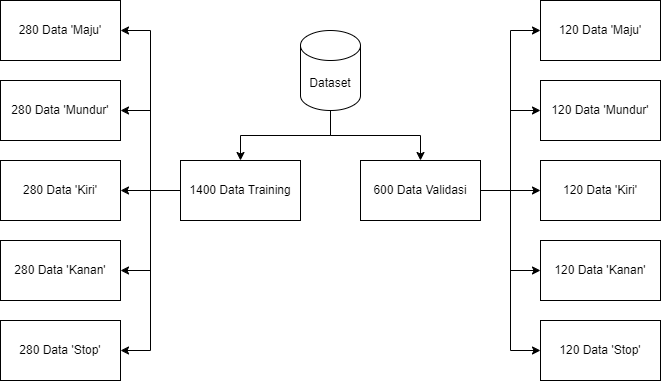
\includegraphics[width=1\textwidth]{gambar/bab4/visualdataset.png}
  % Keterangan gambar yang diinputkan
  \caption{Diagram Pembagian \emph{Dataset}}
  % Label referensi dari gambar yang diinputkan
  \label{fig:dataset}
\end{figure}

%Tabel 4.1
\begin{longtable}{|c|c|c|}
  \caption{\emph{Dataset} Kontrol {Kursi Roda}}
  \label{tb:datadiagram} \\
  \hline
  \rowcolor[HTML]{C0C0C0}
  \textbf{Kelas Kontrol} & \textbf{Data Pelatihan} & \textbf{Data Validasi} \\ \hline
  Kanan            & 280 Citra               & 120 Citra               \\ \hline
  Kiri              & 280 Citra               & 120 Citra               \\ \hline
  Maju             & 280 Citra               & 120 Citra               \\ \hline
  Mundur            & 280 Citra               & 120 Citra               \\ \hline
  Stop             & 280 Citra               & 120 Citra               \\ \hline
\end{longtable}

\subsection{Pengujian Model Pertama}

Dalam pembuatan model pertama, proses pelatihan dilakukan dengan menggunakan model CNN yang terdiri dari delapan lapisan dengan 32 filter pada layer pertama dan 64 filter pada layer kedua. Pelatihan pada model CNN dilakukan dengan konfigurasi 40 tahapan \emph{epoch} dengan 10 langkah pelatihan per \emph{epoch}. Ditambahkan juga modul \emph{early stopping} selama pelatihan model agar didapatkan model terbaik, yaitu pada \emph{epoch} ke-18. Berdasarkan hasil pelatihan tersebut, dihasilkan nilai akurasi sebesar 98\% dengan akurasi validasi sebesar 91.33\%. Selain itu, hasil pelatihan juga menunjukkan nilai \emph{loss} sebesar 9.87\% dengan \emph{loss} validasi sebesar 21.34\%. Variabel tersebut dapat dilihat pada Gambar \ref{fig:acc_loss1} yang telah memvisualisasikan hasil akurasi dan akurasi validasi serta hasil \emph{loss} dan \emph{loss} validasi dalam bentuk grafik dengan nilai akurasi, akurasi validasi, \emph{loss}, dan \emph{loss} validasi terhadap tiap tahapan \emph{epoch}. 

%Gambar 4.2
\begin{figure}[H]
  \centering
  \begin{subfigure}[b]{0.55\textwidth}
      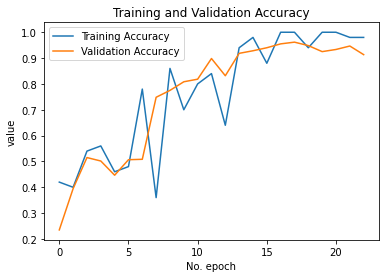
\includegraphics[width=\textwidth]{gambar/bab4/modelpertama/train.png}
      \caption{Akurasi}
  \end{subfigure}

  \begin{subfigure}[b]{0.55\textwidth}
      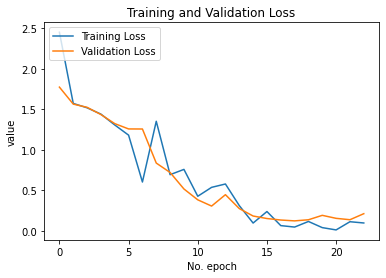
\includegraphics[width=\textwidth]{gambar/bab4/modelpertama/loss.png}
      \caption{\emph{Loss}}
  \end{subfigure}
  \caption{Grafik Akurasi dan \emph{Loss} pada Hasil Pelatihan Model Pertama}
  \label{fig:acc_loss1}
\end{figure}

Setelah didapatkan grafik akurasi dan \emph{loss} untuk hasil pelatihan model, selanjutnya dilakukan perhitungan untuk \emph{confusion matrix}. \emph{Confusion matrix} dihitung dengan membandingkan label yang sebenarnya (\emph{true label}) dengan label yang diprediksi (\emph{predicted label}) yang kemudian kedua label tersebut akan divisualisasikan menjadi \emph{matrix} yang dibagi menjadi tiap kelas kontrol, dimana \emph{predicted label} menjadi sumbu X dan \emph{true label} menjadi sumbu Y. Dari visualisasi \emph{confusion matrix}, dapat diamati bahwa keseluruhan 600 \emph{dataset} validasi yang telah diuji berdasarkan label yang sebenarnya sudah terprediksi dengan benar. \emph{Confusion matrix} yang dihasilkan dapat dilihat pada Gambar \ref{fig:matrix11}.

%Gambar 4.3
\begin{figure} [H] \centering
  % Nama dari file gambar yang diinputkan
  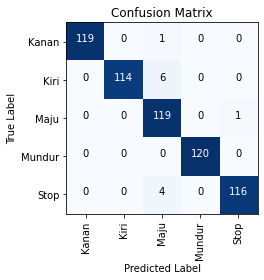
\includegraphics[width=0.35\textwidth]{gambar/bab4/model5 (30cm)/110cm/matrix.png}
  % Keterangan gambar yang diinputkan
  \caption{\emph{Confusion Matrix} Model Pertama}
  % Label referensi dari gambar yang diinputkan
  \label{fig:matrix11}
\end{figure}

Pada Tabel \ref{tb:cm_model1} didapatkan hasil klasifikasi model untuk kelas "Kanan", hasilnya 119 TP dan hanya satu FN, menunjukkan efektivitas tinggi dalam mengenali pose ini. Sementara itu, kelas "Kiri" mengalami sedikit kesulitan dengan 6 FN, mengindikasikan beberapa kasus di mana pose "Kiri" tidak terdeteksi dengan akurat. Untuk kelas "Maju", model ini mengalami 11 FP dan satu FN. Kelas "Mundur" menunjukkan performa yang sangat baik dengan tidak adanya FP atau FN. Akhirnya, untuk kelas "Stop", ada satu FP dan empat FN, yang menunjukkan bahwa beberapa pose "Stop" tidak teridentifikasi sebagai "Stop".

\begin{longtable}{|l|c|c|c|c|}
  \caption{Hasil Klasifikasi Model Pertama}
  \label{tb:cm_model1} \\
  \hline
  \rowcolor[HTML]{C0C0C0} 
  \textbf{Kelas} & \textbf{TP} & \textbf{TN} & \textbf{FP} & \textbf{FN} \\ \hline
  Kanan    & 119          & 480         & 0           & 1           \\ \hline
  Kiri      & 114          & 480         & 0           & 6           \\ \hline
  Maju      & 119          & 469         & 11           & 1           \\ \hline
  Mundur     & 120          & 480         & 0           & 0           \\ \hline
  Stop  & 116          & 479         & 1           & 4           \\ \hline
\end{longtable}

Pada Tabel \ref{tb:vs_model1} berisi hasil validasi untuk kelas "Kanan", model menunjukkan \emph{accuracy} sebesar 99.83\%, \emph{precision} 100\%,\emph{recall} 99.17\%, dan \emph{f1-Score} 99.58\%. Pada kelas "Kiri", model mencatatkan \emph{accuracy 99\%}, \emph{precision} 100\%, \emph{recall} 95\%, dan \emph{f1-Score} 97.44\%. Untuk kelas "Maju", metrik yang tercatat adalah \emph{accuracy} 98\%, \emph{precision} 91.54\%, \emph{recall} 99.17\%, dan \emph{f1-Score} 95.20\%. Kelas "Mundur" menunjukkan performa sempurna dengan 100\% di semua metrik, dan kelas "Stop" memiliki \emph{accuracy} 99.17\%, \emph{precision} 99.15\%, \emph{recall} 96.67\%, serta \emph{f1-Score} 97.89\%. Nilai validasi yang dihitung yaitu \emph{accuracy}, \emph{precision}, \emph{recall}, dan \emph{f-1 score}. 

%Tabel 4.3
\begin{longtable}{|l|c|c|c|c|}
  \caption{Hasil Validasi Model Pertama}
  \label{tb:vs_model1} \\
  \hline
  \rowcolor[HTML]{C0C0C0} 
  \textbf{Kelas} & \textbf{\emph{Accuracy}} & \textbf{\emph{Precision}} & \textbf{\emph{Recall}} & \textbf{\emph{F1-Score}} \\ \hline
  Kanan    & 99.83\%            & 100\%             & 99.17\%           & 99.58\%            \\ \hline
  Kiri     & 99\%          & 100\%           & 95\%           & 97.44\%           \\ \hline
  Maju      & 98\%          & 91.54\%           & 99.17\%          & 95.20\%          \\ \hline
  Mundur     & 100\%            & 100\%             & 100\%           & 100\%            \\ \hline
  Stop  & 99.17\%            & 99.15\%             & 96.67\%           & 97.89\%            \\ \hline
\end{longtable}

\subsection{Pengujian Model Kedua}

Dalam pembuatan model kedua, proses pelatihan dilakukan dengan menggunakan model CNN yang terdiri dari sebelas lapisan dengan 32 filter pada layer pertama, 64 filter pada layer kedua, dan 128 filter pada layer ketiga seperti struktur yang telah dipaparkan pada metodologi penelitian. Pelatihan pada model CNN dilakukan dengan konfigurasi 40 tahapan \emph{epoch} dengan 10 langkah pelatihan per \emph{epoch}. Ditambahkan juga modul \emph{early stopping} selama pelatihan model agar didapatkan model terbaik, yaitu pada \emph{epoch} ke-30. Berdasarkan hasil pelatihan tersebut, dihasilkan nilai akurasi sebesar 100\% dengan akurasi validasi sebesar 99.83\%. Selain itu, hasil pelatihan juga menunjukkan nilai \emph{loss} sebesar 0.22\% dengan \emph{loss} validasi sebesar 1.14\%. Variabel tersebut dapat dilihat pada Gambar \ref{fig:acc_loss} yang telah memvisualisasikan hasil akurasi dan akurasi validasi serta hasil \emph{loss} dan \emph{loss} validasi dalam bentuk grafik dengan nilai akurasi, akurasi validasi, \emph{loss}, dan \emph{loss} validasi terhadap tiap tahapan \emph{epoch}.

%Gambar 4.2
\begin{figure}[H]
  \centering
  \begin{subfigure}[b]{0.55\textwidth}
      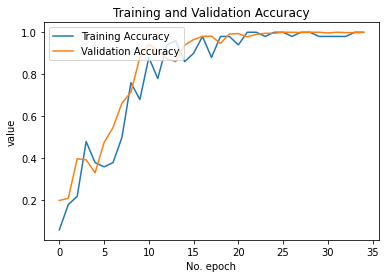
\includegraphics[width=\textwidth]{gambar/bab4/model5 (30cm)/train.png}
      \caption{Akurasi}
  \end{subfigure}

  \begin{subfigure}[b]{0.55\textwidth}
      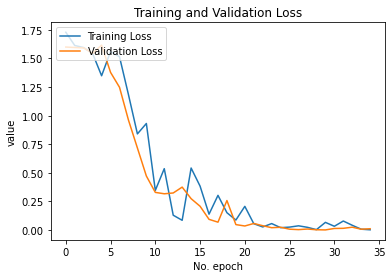
\includegraphics[width=\textwidth]{gambar/bab4/model5 (30cm)/loss.png}
      \caption{\emph{Loss}}
  \end{subfigure}
  \caption{Grafik Akurasi dan \emph{Loss} pada Hasil Pelatihan Model Kedua}
  \label{fig:acc_loss}
\end{figure}

Setelah didapatkan grafik akurasi dan \emph{loss} untuk hasil pelatihan model, selanjutnya dilakukan perhitungan untuk \emph{confusion matrix}. \emph{Confusion matrix} dihitung dengan membandingkan label yang sebenarnya (\emph{true label}) dengan label yang diprediksi (\emph{predicted label}) yang kemudian kedua label tersebut akan divisualisasikan menjadi \emph{matrix} yang dibagi menjadi tiap kelas kontrol, dimana \emph{predicted label} menjadi sumbu X dan \emph{true label} menjadi sumbu Y. Dari visualisasi \emph{confusion matrix}, dapat diamati bahwa terdapat kesalahan prediksi pada kelas "Maju".

%Gambar 4.3
\begin{figure} [H] \centering
  % Nama dari file gambar yang diinputkan
  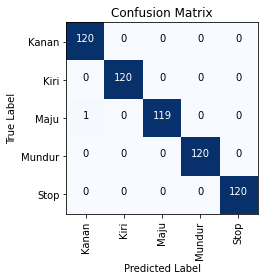
\includegraphics[width=0.35\textwidth]{gambar/bab4/modelkedua/modelkedua.png}
  % Keterangan gambar yang diinputkan
  \caption{\emph{Confusion Matrix} Model Kedua}
  % Label referensi dari gambar yang diinputkan
  \label{fig:matrix1}
\end{figure}

Kemudian dari \emph{confusion matrix}, didapatkan hasil klasifikasi yang dapat dikelompokkan menjadi beberapa parameter yaitu \emph{true positive}, \emph{true negative}, \emph{false positive}, dan \emph{false negative}. \emph{True positive} adalah hasil dimana model memprediksi kelas positif dengan benar. Demikian pula, \emph{true negative} adalah hasil dimana model memprediksi kelas negatif dengan benar. Kelas positif adalah kelas itu sendiri, sedangkan kelas negatif adalah kelas lain selain kelas itu sendiri. \emph{False positive} adalah hasil di mana model salah memprediksi kelas positif. Dan \emph{false negative} adalah hasil di mana model salah memprediksi kelas negatif. Hasil klasifikasi dapat dilihat pada Tabel \ref{tb:cm_model}.

%Tabel 4.2
\begin{longtable}{|l|c|c|c|c|}
  \caption{Hasil Klasifikasi Model Kedua}
  \label{tb:cm_model} \\
  \hline
  \rowcolor[HTML]{C0C0C0} 
  \textbf{Kelas} & \textbf{TP} & \textbf{TN} & \textbf{FP} & \textbf{FN} \\ \hline
  Kanan    & 120          & 479         & 1           & 0           \\ \hline
  Kiri      & 120          & 480         & 0           & 0           \\ \hline
  Maju      & 119          & 480         & 0           & 1           \\ \hline
  Mundur     & 120          & 480         & 0           & 0           \\ \hline
  Stop  & 120          & 480         & 0           & 0           \\ \hline
\end{longtable}

Berdasarkan Tabel \ref{tb:cm_model} diatas, dapat dilihat pada kelas "Kiri", "Mundur", dan "Stop" memiliki 120 data citra yang termasuk dalam \emph{true positive}, 480 data citra yang termasuk dalam \emph{true negative}, 0 data citra yang termasuk dalam \emph{false positive}, dan 0 data citra yang termasuk dalam \emph{false negative}. Sedangkan pada kelas "Kanan" terdapat 1 data citra yang termasuk dalam \emph{false positive} dan kelas "Maju" terdapat 1 data citra yang termasuk dalam \emph{false negative}, hal tersebut menunjukkan bahwa terdapat kesalahan deteksi pada "Maju" yang diangggap sebagai kelas "Kanan". Dari hasil klasifikasi tersebut, selanjutnya dapat dihitung nilai validasi model. Nilai validasi yang dihitung yaitu \emph{accuracy}, \emph{precision}, \emph{recall}, dan \emph{f-1 score}. Penggambaran lebih detail dapat dilihat pada Tabel \ref{tb:vs_model}. 

%Tabel 4.3
\begin{longtable}{|l|c|c|c|c|}
  \caption{Hasil Validasi Model Kedua}
  \label{tb:vs_model} \\
  \hline
  \rowcolor[HTML]{C0C0C0} 
  \textbf{Kelas} & \textbf{\emph{Accuracy}} & \textbf{\emph{Precision}} & \textbf{\emph{Recall}} & \textbf{\emph{F1-Score}} \\ \hline
  Kanan    & 99.83\%            & 99.17\%             & 100\%           & 99.59\%            \\ \hline
  Kiri     & 100\%          & 100\%           & 100\%           & 100\%           \\ \hline
  Maju      & 99.83\%          & 100\%           & 99.17\%          & 99.58\%          \\ \hline
  Mundur     & 100\%            & 100\%             & 100\%           & 100\%            \\ \hline
  Stop  & 100\%            & 100\%             & 100\%           & 100\%            \\ \hline
\end{longtable}

Dapat dilihat dari Tabel \ref{tb:vs_model}, nilai \emph{accuracy}, \emph{precision}, \emph{recall}, dan \emph{f1-score} untuk kelas "Kanan" , didapatkan nilai \emph{accuracy} sebesar 99.83\%, nilai \emph{precision} sebesar 99.17\%, nilai \emph{recall} sebesar 100\%, dan nilai \emph{f1-score} sebesar 99.59\%. Kemudian untuk kelas "Kiri" , didapatkan nilai \emph{accuracy} sebesar 100\%, nilai \emph{precision} sebesar 100\%, nilai \emph{recall} sebesar 100\%, dan nilai \emph{f1-score} sebesar 100\%. Selanjutnya pada kelas "Maju" , didapatkan nilai \emph{accuracy} sebesar 99.83\%, nilai \emph{precision} sebesar 100\%, nilai \emph{recall} sebesar 99.17\%, dan nilai \emph{f1-score} sebesar 99.58\%. Untuk kelas "Mundur" , didapatkan nilai \emph{accuracy} sebesar 100\%, nilai \emph{precision} sebesar 100\%, nilai \emph{recall} sebesar 100\%, dan nilai \emph{f1-score} sebesar 100\%. Terakhir pada kelas "Stop" , didapatkan nilai \emph{accuracy} sebesar 100\%, nilai \emph{precision} sebesar 100\%, nilai \emph{recall} sebesar 100\%, dan nilai \emph{f1-score} sebesar 100\%. Nilai validasi tersebut bisa didapatkan karena nilai \emph{true positive}, \emph{true negative}, \emph{false positive}, dan \emph{false negative} dari \emph{confusion matrix} yang dipaparkan pada Tabel \ref{tb:cm_model} memiliki nilai prediksi yang baik untuk kelima kelas. Karena model kedua memiliki performa yang lebih baik dibandingkan dengan model pertama, maka model kedua dipilih sebagai model yang akan digunakan dalam pengujian selanjutnya.

\section{Pengujian Performa Model dengan menggunakan Variasi Jarak}

Pada skenario pengujian selanjutnya, model diuji berdasarkan beberapa variasi jarak. Pengujian jarak berguna untuk mengetahui performa dan tingkat akurasi model jika input citra diambil dari jarak yang berbeda-beda. Hal ini perlu diuji karena semakin jauh jarak pendeteksi citra, maka semakin kecil data visual citra yang diperoleh. Variasi jarak yang digunakan adalah 30 sentimeter, 50 sentimeter, 70 sentimeter, dan 90 sentimeter. Contoh \emph{dataset} untuk pengujian variasi jarak dapat dilihat pada Gambar \ref{fig:Variasi Jarak}.

\begin{figure}[H]
  \centering
  \begin{subfigure}[b]{0.4\linewidth}
      
\includegraphics[width=\linewidth]{gambar/bab4/30.jpg}
      \caption{Jarak 30 sentimeter}
      \label{fig:imageaa}
  \end{subfigure}
  \hfill % adds horizontal space between the figures
  \begin{subfigure}[b]{0.4\linewidth}
    
\includegraphics[width=\linewidth]{gambar/bab4/50.jpg}
    \caption{Jarak 50 sentimeter}
    \label{fig:imagebb}
  \end{subfigure}
  \vspace{1cm} % adds vertical space between the rows of images
  \begin{subfigure}[b]{0.4\linewidth}
    
\includegraphics[width=\linewidth]{gambar/bab4/70.jpg}
    \caption{Jarak 70 sentimeter}
    \label{fig:imagecc}
  \end{subfigure}
  \begin{subfigure}[b]{0.4\linewidth}
    
\includegraphics[width=\linewidth]{gambar/bab4/90.jpg}
    \caption{Jarak 90 sentimeter}
    \label{fig:imagedd}
  \end{subfigure}
  \caption{Variasi \emph{Dataset} Pengujian Jarak}
  \label{fig:Variasi Jarak}
\end{figure}

Model diuji menggunakan \emph{dataset} validasi yang terdiri dari 600 data citra yang dibagi rata sebanyak 120 data citra yang dikelompokkan ke dalam lima kelas. Pengujian model dihitung dengan menggunakan \emph{confusion matrix}. Yang kemudian, dari \emph{confusion matrix} didapatkan nilai \emph{true positive} (TP), \emph{true negative} (TN), \emph{false positive} (FP), dan \emph{false negative} (FN) dari masing-masing kelas yang diuji. Selanjutnya dari keempat variabel tersebut, dapat dihitung \emph{accuracy}, \emph{precision}, \emph{recall}, dan \emph{f-1 score}. Nilai-nilai ini mencerminkan seberapa baik model mampu mengidentifikasi kelas yang benar \emph{(recall)}, seberapa akurat prediksi yang diberikan \emph{(precision)}, serta keseimbangan antara keduanya melalui \emph{f-1 score}. 

\subsection{Jarak 30 sentimeter}

Skenario pengujian jarak yang pertama dilakukan dengan jarak 30 sentimeter dari kamera ke objek deteksi. Berdasarkan \emph{confusion matrix} pada Gambar \ref{fig:matrix2} dapat diamati bahwa hasil pengujian dengan jarak 30 sentimeter memiliki hasil prediksi yang akurat pada semua kelas dimana semua label yang diprediksi sesuai dengan semua label yang sebenarnya.

%Gambar 4.4
\begin{figure} [H] \centering
  % Nama dari file gambar yang diinputkan
  \includegraphics[width=0.35\textwidth]{gambar/bab4/model5 (30cm)/matrix.png}
  % Keterangan gambar yang diinputkan
  \caption{\emph{Confusion Matrix} Model dengan Jarak 30 cm}
  % Label referensi dari gambar yang diinputkan
  \label{fig:matrix2}
\end{figure}

Kemudian dari \emph{confusion matrix} yang didapat, diperoleh nilai TP, TN, FP, dan FN seperti yang tertera pada Tabel \ref{tb:cm_model2}. Dapat dilihat bahwa pada semua kelas, nilai TP yang diperoleh sebanyak 120 data citra, nilai TN sebanyak 480 data citra, nilai FP sebanyak 0 data citra, dan nilai FN sebanyak 0 data citra yang menunjukkan bahwa model dapat mengenali perbedaan antara kelas dengan akurasi tinggi, dan mampu mendeteksi kelas yang benar setiap kali diberikan input pada jarak 30 sentimeter.

%Tabel 4.4
\begin{longtable}{|l|c|c|c|c|}
  \caption{Hasil Klasifikasi Model dengan Jarak 30 cm}
  \label{tb:cm_model2} \\
  \hline
  \rowcolor[HTML]{C0C0C0} 
  \textbf{Kelas} & \textbf{TP} & \textbf{TN} & \textbf{FP} & \textbf{FN} \\ \hline
  Kanan    & 120          & 480         & 0           & 0           \\ \hline
  Kiri      & 120          & 480         & 0           & 0           \\ \hline
  Maju      & 120          & 480         & 0           & 0           \\ \hline
  Mundur     & 120          & 480         & 0           & 0           \\ \hline
  Stop  & 120          & 480         & 0           & 0           \\ \hline
\end{longtable}

Dari nilai TP, TN , FP, dan FN diatas, dapat dihitung nilai \emph{accuracy}, \emph{precision}, \emph{recall}, dan \emph{f-1 score} seperti yang tertera pada Tabel \ref{tb:vs_model2}. Pada semua kelas, didapat nilai \emph{accuracy} sebesar 100\%, nilai \emph{precision} sebesar 100\%, nilai \emph{recall} sebesar 100\%, dan nilai \emph{f-1 score} sebesar 100\%. Keempat variabel tersebut dapat bernilai bagus karena hasil perhitungannya berbanding lurus dengan perhitungan \emph{confusion matrix}. 

Nilai-nilai ini menunjukkan bahwa model dapat mengenali perbedaan antara kelas dengan akurasi tinggi, dan mampu mendeteksi kelas yang benar setiap kali diberikan input pada jarak 30 sentimeter. Selain itu, keempat variabel tersebut dapat bernilai bagus karena hasil perhitungannya berbanding lurus dengan perhitungan \emph{confusion matrix}. 

%Tabel 4.5
\begin{longtable}{|l|c|c|c|c|}
  \caption{Hasil Validasi Model dengan Jarak 30 cm}
  \label{tb:vs_model2} \\
  \hline
  \rowcolor[HTML]{C0C0C0} 
  \textbf{Kelas} & \textbf{\emph{Accuracy}} & \textbf{\emph{Precision}} & \textbf{\emph{Recall}} & \textbf{\emph{F1-Score}} \\ \hline
  Kanan    & 100\%            & 100\%             & 100\%           & 100\%            \\ \hline
  Kiri     & 100\%          & 100\%           & 100\%           & 100\%           \\ \hline
  Maju      & 100\%          & 100\%           & 100\%          & 100\%          \\ \hline
  Mundur     & 100\%            & 100\%             & 100\%           & 100\%            \\ \hline
  Stop  & 100\%            & 100\%             & 100\%           & 100\%            \\ \hline
\end{longtable}

\subsection{Jarak 50 sentimeter}

Selanjutnya, pengujian dilakukan dengan variasi jarak 50 sentimeter. Dari data pada \emph{confusion matrix} di Gambar \ref{fig:matrix3}, dapat dilihat bahwa setiap kelas memiliki 120 prediksi yang benar dan tidak terdapat kesalahan klasifikasi antarkelas mana pun. Setiap nilai diagonal yang mencapai 120 mengindikasikan bahwa semua prediksi untuk kelas tersebut sesuai dengan label sebenarnya. 

%Gambar 4.5
\begin{figure} [H] \centering
  % Nama dari file gambar yang diinputkan
  \includegraphics[width=0.35\textwidth]{gambar/bab4/model6 (50cm)/matrix.png}
  % Keterangan gambar yang diinputkan
  \caption{\emph{Confusion Matrix} Model dengan Jarak 50 cm}
  % Label referensi dari gambar yang diinputkan
  \label{fig:matrix3}
\end{figure}

Pada Tabel \ref{tb:cm_model3} yang disajikan menampilkan hasil pengujian model klasifikasi yang digunakan untuk mengendalikan kursi roda melalui pose mata dari jarak 50 sentimeter. Untuk semua kelas, angka \emph{True Positive} mencatat 120, menunjukkan bahwa model secara konsisten berhasil mengidentifikasi setiap pose dengan benar sebanyak 120 kali. \emph{True Negative}, yang juga mencapai 480 untuk setiap kelas, mengindikasikan bahwa model sangat efisien dalam tidak salah mengklasifikasikan pose lain sebagai pose yang sedang diuji. Sementara itu, nilai untuk \emph{False Positive} dan \emph{False Negative} adalah nol, menunjukkan bahwa tidak ada kesalahan dalam pengklasifikasian pose. Secara keseluruhan, tabel ini menggambarkan performa yang sangat baik dari model dalam mengklasifikasikan pose mata dari jarak 50 sentimeter.

%Tabel 4.6
\begin{longtable}{|l|c|c|c|c|}
  \caption{Hasil Klasifikasi Model dengan Jarak 50 cm}
  \label{tb:cm_model3} \\
  \hline
  \rowcolor[HTML]{C0C0C0} 
  \textbf{Kelas} & \textbf{TP} & \textbf{TN} & \textbf{FP} & \textbf{FN} \\ \hline
  Kanan    & 120          & 480         & 0           & 0           \\ \hline
  Kiri      & 120          & 480         & 0           & 0           \\ \hline
  Maju      & 120          & 480         & 0           & 0           \\ \hline
  Mundur     & 120          & 480         & 0           & 0           \\ \hline
  Stop  & 120          & 480         & 0           & 0           \\ \hline
\end{longtable}

Berdasarkan nilai TP, TN, FP, dan FN yang didapatkan, dapat didapatkan nilai 100\% di semua metrik evaluasi—\emph{Accuracy, Precision, Recall}, dan \emph{F1-Score}—untuk kelima kelas: "Kanan", "Kiri", "Maju", "Mundur", dan "Stop" pada jarak 50 sentimeter. Akurasi sempurna menunjukkan tidak adanya kesalahan dalam klasifikasi, sementara presisi 100\% mengindikasikan tidak ada FP, dan \emph{recall} 100\% menandakan model berhasil menangkap semua kasus positif sebenarnya tanpa kehilangan satu pun. Skor F1 yang juga sempurna menunjukkan keseimbangan optimal antara presisi dan \emph{recall}.

%Tabel 4.7
\begin{longtable}{|l|c|c|c|c|}
  \caption{Hasil Validasi Model dengan Jarak 50 cm}
  \label{tb:vs_model3} \\
  \hline
  \rowcolor[HTML]{C0C0C0} 
  \textbf{Kelas} & \textbf{\emph{Accuracy}} & \textbf{\emph{Precision}} & \textbf{\emph{Recall}} & \textbf{\emph{F1-Score}} \\ \hline
  Kanan    & 100\%            & 100\%             & 100\%           & 100\%            \\ \hline
  Kiri     & 100\%          & 100\%           & 100\%           & 100\%           \\ \hline
  Maju      & 100\%          & 100\%           & 100\%          & 100\%          \\ \hline
  Mundur     & 100\%            & 100\%             & 100\%           & 100\%            \\ \hline
  Stop  & 100\%            & 100\%             & 100\%           & 100\%            \\ \hline
\end{longtable}

\subsection{Jarak 70 sentimeter}

Pada tahap pengujian berikutnya, dilakukan pengujian model dengan jarak 70 sentimeter. Dari \emph{confusion matrix} pada Gambar \ref{fig:matrix5}, dapat diamati performa model secara keseluruhan sangat baik dengan setiap kelas kecuali "Maju". Pada kelas "Maju", terlihat bahwa model berhasil mengidentifikasi 117 kasus dengan benar namun, ada 3 kasus yang keliru diidentifikasi sebagai "Mundur", menunjukkan sedikit kelemahan dalam membedakan antara dua pose ini.

%Gambar 4.7
\begin{figure} [H] \centering
  % Nama dari file gambar yang diinputkan
  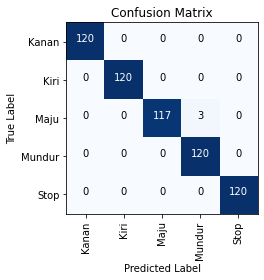
\includegraphics[width=0.35\textwidth]{gambar/bab4/model8 (90cm)/matrix.png}
  % Keterangan gambar yang diinputkan
  \caption{\emph{Confusion Matrix} Model dengan Jarak 70 cm}
  % Label referensi dari gambar yang diinputkan
  \label{fig:matrix5}
\end{figure}

Pada Tabel \ref{tb:cm_model5}, untuk kelas "Kanan", "Kiri", dan "Stop", model mencapai nilai TP maksimal yaitu 120, dengan TN 480, dan FP atau FN, menandakan tidak ada kesalahan klasifikasi. Untuk kelas "Maju" menunjukkan 117 TP dan 3 FN, yang berarti ada tiga kasus di mana pose Maju tidak diidentifikasi dengan benar. Untuk kelas "Mundur", terdapat sedikit gangguan di mana meskipun mendapat 120 TP, terdapat 3 FP yang berarti model salah mengklasifikasikan tiga pose lain sebagai "Mundur".

%Tabel 4.8
\begin{longtable}{|l|c|c|c|c|}
  \caption{Hasil Klasifikasi Model dengan Jarak 70 cm}
  \label{tb:cm_model5} \\
  \hline
  \rowcolor[HTML]{C0C0C0} 
  \textbf{Kelas} & \textbf{TP} & \textbf{TN} & \textbf{FP} & \textbf{FN} \\ \hline
  Kanan    & 120          & 480         & 0           & 0           \\ \hline
  Kiri      & 120          & 480         & 0           & 0           \\ \hline
  Maju      & 117          & 480         & 0           & 3           \\ \hline
  Mundur     & 120          & 477         & 3           & 0           \\ \hline
  Stop  & 120          & 480         & 0           & 0           \\ \hline
\end{longtable}


Pada Tabel \ref{tb:vs_model5}, untuk kelas "Maju", model menunjukkan hasil dengan \emph{Accuracy} sebesar 99.50\%, \emph{Precision} 100\%, \emph{Recall} 97.50\%, dan \emph{F1-Score} 98.73\%. Untuk kelas "Mundur", model mencatat \emph{Accuracy} 99.50\%, namun dengan \emph{Precision} sedikit menurun menjadi 97.56\%, yang mencerminkan adanya beberapa kesalahan dalam memprediksi pose sebagai "Mundur". Namun, dengan \emph{Recall} 100\% dan \emph{F1-Score} 98.77\%, dapat dilihat bahwa model tersebut secara konsisten mengidentifikasi semua pose "Mundur" yang sebenarnya. Secara keseluruhan, hasil ini menunjukkan bahwa model memiliki performa yang baik dalam mengenali kedua pose tersebut.

%Tabel 4.9
\begin{longtable}{|l|c|c|c|c|}
  \caption{Hasil Validasi Model dengan Jarak 70 cm}
  \label{tb:vs_model5} \\
  \hline
  \rowcolor[HTML]{C0C0C0} 
  \textbf{Kelas} & \textbf{\emph{Accuracy}} & \textbf{\emph{Precision}} & \textbf{\emph{Recall}} & \textbf{\emph{F1-Score}} \\ \hline
  Kanan    & 100\%            & 100\%             & 100\%           & 100\%            \\ \hline
  Kiri     & 100\%          & 100\%           & 100\%           & 100\%           \\ \hline
  Maju      & 99.50\%          & 100\%           & 97.50\%          & 98.73\%          \\ \hline
  Mundur     & 99.50\%            & 97.56\%             & 100\%           & 98.77\%            \\ \hline
  Stop  & 100\%            & 100\%             & 100\%           & 100\%            \\ \hline
\end{longtable}

\subsection{Jarak 90 sentimeter}

Skenario pengujian jarak yang terakhir adalah dengan jarak 90 sentimeter dari kamera ke objek yang dijadikan data citra. Melalui analisis \emph{confusion matrix} pada Gambar \ref{fig:matrix6} untuk kelas "Maju", model berhasil mengidentifikasi 106 dari 120 pose dengan benar, dengan 14 pose diklasifikasikan sebagai "Mundur". Untuk kelas "Mundur", model menunjukkan kelemahan yang lebih signifikan dengan 114 pose yang diklasifikasikan dengan benar dan 6 pose yang salah diklasifikasikan sebagai "Maju". 

Hal ini menunjukkan kesulitan model dalam membedakan antara pose "Maju" dan "Mundur". Sementara itu, kelas "Kanan", "Kiri", dan "Stop" memiliki tingkat akurasi yang tinggi yaitu semua 120 pose terdeteksi dengan benar. Kesalahan ini mungkin disebabkan oleh kemiripan pose atau penurunan akurasi deteksi karena peningkatan jarak, sebab semakin jauh jarak maka semakin kecil data citra yang didapat. 
  
%Gambar 4.8
\begin{figure} [H] \centering
  % Nama dari file gambar yang diinputkan
  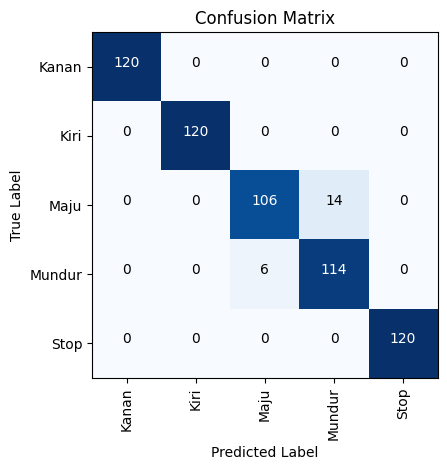
\includegraphics[width=0.35\textwidth]{gambar/bab4/model8 (90cm)/confusion.png}
  % Keterangan gambar yang diinputkan
  \caption{\emph{Confusion Matrix} Model dengan Jarak 90 cm}
  % Label referensi dari gambar yang diinputkan
  \label{fig:matrix6}
\end{figure}

Dari hasil perhitungan \emph{confusion matrix} didapatkan hasil klasifikasi model pada Tabel \ref{tb:cm_model6}. Untuk kelas "Kanan", "Kiri", dan "Stop" menghasilkan 120 TP, menunjukkan efektivitas tinggi dalam mengenali pose ini. Sementara itu, untuk kelas "Maju", model ini memiliki 106 TP, 474 TN, 6 FP,dan 14 FN. Kelas Mundur menunjukkan 114 TP, 466 TN, 14 FP, dan 6 FN menunjukkan sedikit kesalahan dalam mengklasifikasikan antara pose Maju dan Mundur.  

%Tabel 4.10
\begin{longtable}{|l|c|c|c|c|}
  \caption{Hasil Klasifikasi Model dengan Jarak 90 cm}
  \label{tb:cm_model6} \\
  \hline
  \rowcolor[HTML]{C0C0C0} 
  \textbf{Kelas} & \textbf{TP} & \textbf{TN} & \textbf{FP} & \textbf{FN} \\ \hline
  Kanan    & 120          & 480         & 0           & 0           \\ \hline
  Kiri      & 120          & 480         & 0           & 0           \\ \hline
  Maju      & 106          & 474         & 6           & 14           \\ \hline
  Mundur     & 114          & 466         & 14           & 6           \\ \hline
  Stop  & 120          & 480         & 0           & 0           \\ \hline
\end{longtable}

Pada Tabel \ref{tb:vs_model6} berisi hasil validasi untuk setiap kelas dalam model. Untuk kelas "Kanan", model menunjukkan \textit{Accuracy} sebesar 100\%, \textit{Precision} 100\%, \textit{Recall} 100\%, dan \textit{F1-Score} 100\%. Pada kelas "Kiri", model mencatatkan \textit{Accuracy} 100\%, \textit{Precision} 100\%, \textit{Recall} 100\%, dan \textit{F1-Score} 100\%. Untuk kelas "Maju", metrik yang tercatat adalah \textit{Accuracy} 96.67\%, \textit{Precision} 94.64\%, \textit{Recall} 88.33\%, dan \textit{F1-Score} 91.38\%. Kelas "Mundur" memiliki memiliki \textit{Accuracy} 96.67\%, \textit{Precision} 89.06\%, \textit{Recall} 95\%, serta \textit{F1-Score} 91.94\%, dan kelas "Stop" memiliki \textit{Accuracy} 100\%, \textit{Precision} 100\%, \textit{Recall} 100\%, serta \textit{F1-Score} 100\%.

%Tabel 4.11
\begin{longtable}{|l|c|c|c|c|}
  \caption{Hasil Validasi Model dengan Jarak 90 cm}
  \label{tb:vs_model6} \\
  \hline
  \rowcolor[HTML]{C0C0C0} 
  \textbf{Kelas} & \textbf{\emph{Accuracy}} & \textbf{\emph{Precision}} & \textbf{\emph{Recall}} & \textbf{\emph{F1-Score}} \\ \hline
  Kanan    & 100\%            & 100\%             & 100\%           & 100\%            \\ \hline
  Kiri     & 100\%          & 100\%           & 100\%           & 100\%           \\ \hline
  Maju      & 96.67\%          & 94.64\%           & 88.33\%          & 91.38\%          \\ \hline
  Mundur     & 96.67\%            & 89.06\%             & 95\%           & 91.94\%            \\ \hline
  Stop  & 100\%            & 100\%             & 100\%           & 100\%            \\ \hline
\end{longtable}

Pengujian performa model dengan variasi jarak menunjukkan tren yang jelas bahwa semakin jauh jarak, performa model semakin berkurang. Hal ini dibuktikan dengan penurunan nilai \emph{accuracy, precision, recall, dan f1 score} seiring bertambahnya jarak. Hasil pengujian ini menegaskan bahwa jarak antara kamera dan pengguna memiliki pengaruh yang signifikan terhadap performa model. Model bekerja paling optimal pada jarak 30 sentimeter dan 50 sentimeter, sedangkan jarak yang lebih jauh seperti 70 sentimeter dan 90 sentimeter performa model menjadi kurang optimal terutama pada kelas "Maju" dan kelas "Mundur". Dengan demikian, pemilihan jarak yang ideal menjadi penting dalam implementasi sistem kontrol kursi roda berbasis pose mata.

\section{Pengujian Performa Model dengan menggunakan Variasi Pencahayaan}

Pada sistem kontrol kursi roda berbasis pose mata, variasi pencahayaan memiliki pengaruh signifikan terhadap performa deteksi model. Model harus mampu beroperasi dalam berbagai kondisi pencahayaan. Sub-bab ini akan membahas pengujian performa model dengan menggunakan variasi pencahayaan. Tujuan dari pengujian ini adalah untuk mengevaluasi tingkat keberhasilan dan ketidakberhasilan model dalam mendeteksi pose mata pada tiga kondisi pencahayaan, yaitu pencahayaan gelap (35 Lux), pencahayaan redup (55 Lux), dan pencahayaan terang (131 Lux). Contoh \emph{dataset} pengujian variasi pencahayaan dapat dilihat pada Gambar \ref{fig:Variasi Lux}.

\begin{figure}[H]
  \centering
  \begin{subfigure}[b]{0.4\linewidth}
      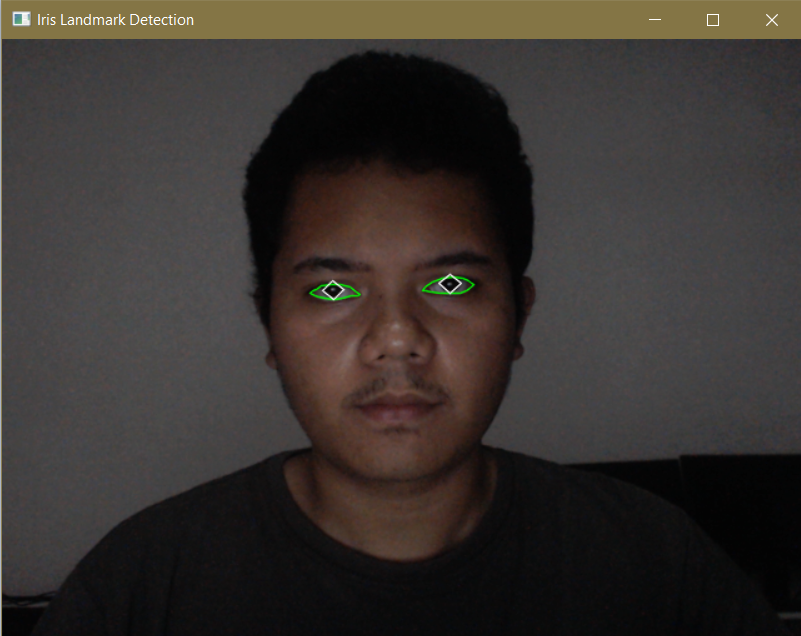
\includegraphics[width=\linewidth]{gambar/bab4/33.png}
      \caption{35 Lux}
      \label{fig:imagea}
  \end{subfigure}
  \hfill % adds horizontal space between the figures
  \begin{subfigure}[b]{0.4\linewidth}
      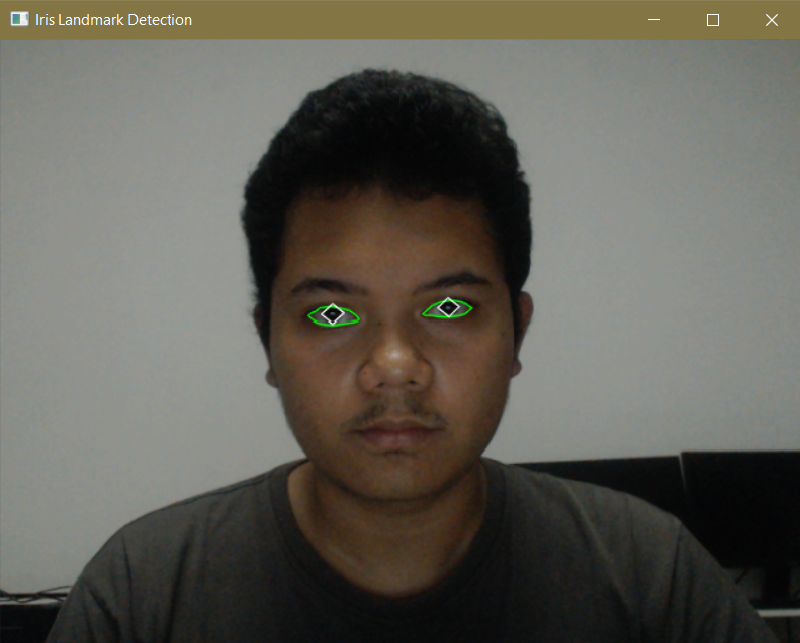
\includegraphics[width=\linewidth]{gambar/bab4/55.png}
      \caption{55 Lux}
      \label{fig:imageb}
  \end{subfigure}
  \vspace{1cm} % adds vertical space between the rows of images
  \begin{subfigure}[b]{0.4\linewidth}
      \centering % centers the image
      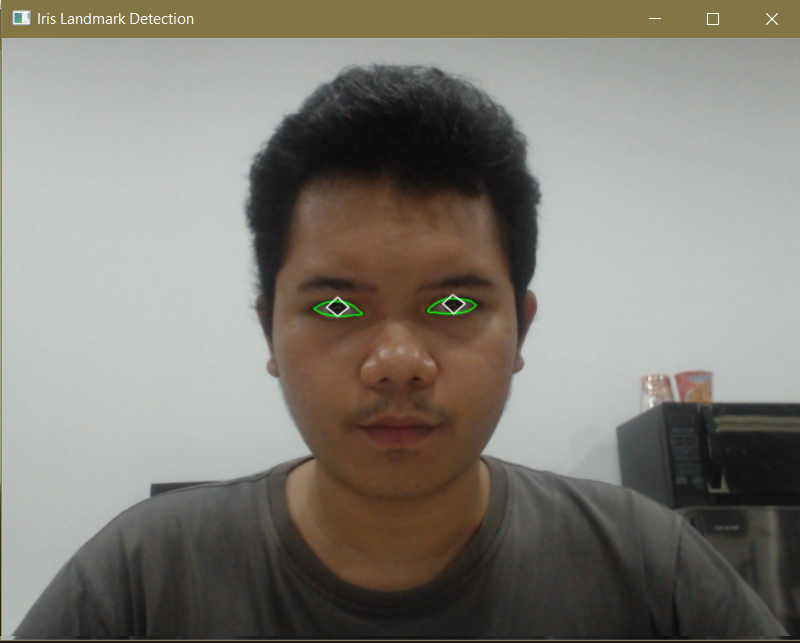
\includegraphics[width=\linewidth]{gambar/bab4/131.png}
      \caption{131 Lux}
      \label{fig:imagec}
  \end{subfigure}
  \caption{Variasi \emph{Dataset} Pengujian Pencahayaan}
  \label{fig:Variasi Lux}
\end{figure}

Jenis pencahayaan yang diuji adalah \emph{ambient light}, yang mensimulasikan pencahayaan lingkungan sekitar dengan variasi intensitas yang berbeda. \emph{Ambient light} adalah pencahayaan umum yang ada di sekitar lingkungan, yang dapat berasal dari sumber cahaya alami seperti sinar matahari atau buatan seperti lampu. Tingkat keberhasilan dan ketidakberhasilan dihitung dalam persentase, dengan data yang dikumpulkan selama tiga puluh sesi pengujian. Hasil dari analisis ini akan memberikan gambaran mengenai seberapa baik model dapat beradaptasi terhadap variasi pencahayaan yang berbeda.

\subsection{Pencahayaan 35 Lux}

Pengujian pada kondisi pencahayaan 35 lux bertujuan untuk mengevaluasi performa model dalam mendeteksi pose mata pada situasi pencahayaan yang gelap. Kondisi ini mensimulasikan lingkungan dengan cahaya minimal yaitu di ruangan yang hanya diterangi lampu yang gelap. Pada pengujian ini ditunjukkan kemampuan model dalam mengeksekusi perintah kontrol pada pencahayaan rendah. Hasil pengujian ini akan memberikan gambaran mengenai kemampuan model dalam mengenali pose mata pada kondisi pencahayaan yang gelap. Selain itu, pengujian ini juga penting untuk memastikan bahwa model tetap berfungsi dengan baik di bawah kondisi pencahayaan yang tidak ideal, yang sering kali terjadi dalam penggunaan sehari-hari.

%Tabel 4.12
\begin{longtable}{|l|c|c|c|c|}
  \caption{Pengujian Kinerja Model dengan Pencahayaan 35 Lux}
  \label{tb:lux35} \\
  \hline
  \rowcolor[HTML]{C0C0C0} 
  \textbf{Kelas} & \multicolumn{1}{c|}{\textbf{\begin{tabular}[c]{@{}c@{}}Jumlah \\ Keberhasilan\end{tabular}}} & \multicolumn{1}{c|}{\textbf{\begin{tabular}[c]{@{}c@{}}Jumlah \\ Ketidakberhasilan\end{tabular}}} & \multicolumn{1}{c|}{\textbf{\begin{tabular}[c]{@{}c@{}}Persentase \\ Keberhasilan\end{tabular}}} & \multicolumn{1}{c|}{\textbf{\begin{tabular}[c]{@{}c@{}}Persentase\\ Ketidakberhasilan\end{tabular}}} \\ \hline
  Kanan  & 30                                                                                  & 0                                                                                        & 100\%                                                                                   & 0\%                                                                                         \\ \hline
  Kiri   & 30                                                                                  & 0                                                                                        & 100\%                                                                                   & 0\%                                                                                         \\ \hline
  Maju   & 27                                                                                  & 3                                                                                        & 90\%                                                                                    & 10\%                                                                                        \\ \hline
  Mundur & 28                                                                                  & 2                                                                                        & 93.33\%                                                                                 & 6.67\%                                                                                      \\ \hline
  Stop   & 30                                                                                  & 0                                                                                        & 100\%                                                                                   & 0\%                                                                                         \\ \hline
\end{longtable}

Berdasarkan hasil pengujian performa model dengan variasi pencahayaan 35 Lux pada Tabel \ref{tb:lux35}, model menunjukkan tingkat keberhasilan yang sempurna pada kelas "Kanan", "Kiri", dan "Stop" dengan masing-masing tingkat keberhasilan 100\%. Namun, pada kelas "Maju", tingkat keberhasilan sebesar 90\% dengan 3 kesalahan deteksi (10\%), dan pada kelas "Mundur", tingkat keberhasilan 93.33\% dengan 2 kesalahan deteksi (6.67\%). Hasil ini menunjukkan bahwa meskipun model umumnya memiliki performa yang baik, akurasi deteksi pada kelas "Maju" dan "Mundur" dipengaruhi oleh variasi pencahayaan.

\subsection{Pencahayaan 55 Lux}

Pada bagian ini, akan dianalisis bagaimana model beroperasi di bawah pencahayaan sebesar 55 Lux. Pencahayaan ini mensimulasikan kondisi ruangan yang redup. Pengujian ini bertujuan untuk memastikan bahwa model dapat mendeteksi dan mengklasifikasikan pose mata dengan akurasi tinggi dalam kondisi pencahayaan redup. Hasil pengujian ini akan memberikan gambaran mengenai kemampuan model beradaptasi dengan baik terhadap variasi pencahayaan dalam lingkungan sehari-hari. Selain itu, analisis ini juga akan membantu dalam mengidentifikasi potensi kelemahan model yang mungkin perlu diperbaiki untuk meningkatkan kinerja secara keseluruhan dalam berbagai kondisi pencahayaan. Dengan demikian, kita dapat mengembangkan solusi yang lebih \emph{robust} untuk aplikasi di dunia nyata.

%Tabel 4.13
\begin{longtable}{|l|c|c|c|c|}
  \caption{Pengujian Kinerja Model dengan Pencahayaan 55 Lux}
  \label{tb:lux55} \\
  \hline
  \rowcolor[HTML]{C0C0C0} 
  \textbf{Kelas} & \multicolumn{1}{c|}{\textbf{\begin{tabular}[c]{@{}c@{}}Jumlah \\ Keberhasilan\end{tabular}}} & \multicolumn{1}{c|}{\textbf{\begin{tabular}[c]{@{}c@{}}Jumlah \\ Ketidakberhasilan\end{tabular}}} & \multicolumn{1}{c|}{\textbf{\begin{tabular}[c]{@{}c@{}}Persentase \\ Keberhasilan\end{tabular}}} & \multicolumn{1}{c|}{\textbf{\begin{tabular}[c]{@{}c@{}}Persentase\\ Ketidakberhasilan\end{tabular}}} \\ \hline
  \endfirsthead
  
  \caption[]{Pengujian Kinerja Model dengan Pencahayaan 55 Lux \textit{(Lanjutan...)}} \\
  \hline
  \rowcolor[HTML]{C0C0C0} 
  \textbf{Kelas} & \multicolumn{1}{c|}{\textbf{\begin{tabular}[c]{@{}c@{}}Jumlah \\ Keberhasilan\end{tabular}}} & \multicolumn{1}{c|}{\textbf{\begin{tabular}[c]{@{}c@{}}Jumlah \\ Ketidakberhasilan\end{tabular}}} & \multicolumn{1}{c|}{\textbf{\begin{tabular}[c]{@{}c@{}}Persentase \\ Keberhasilan\end{tabular}}} & \multicolumn{1}{c|}{\textbf{\begin{tabular}[c]{@{}c@{}}Persentase\\ Ketidakberhasilan\end{tabular}}} \\ \hline
  \endhead

  \hline
  \multicolumn{5}{r}{\textit{(Tabel bersambung...)}} \\
  \endfoot

  \hline
  \endlastfoot

  Kanan  & 30 & 0 & 100\% & 0\% \\ \hline
  Kiri   & 30 & 0 & 100\% & 0\% \\ \hline
  Maju   & 29 & 1 & 96.67\% & 3.33\% \\ \hline
  Mundur & 28 & 2 & 93.33\% & 6.67\% \\ \hline
  Stop   & 30 & 0 & 100\% & 0\% \\ \hline
\end{longtable}

Pada Tabel \ref{tb:lux55}, pengujian kinerja model dengan pencahayaan 55 Lux, hasil menunjukkan bahwa model secara umum memiliki tingkat akurasi yang baik. Perintah "Kanan", "Kiri", dan "Stop" mencapai tingkat keberhasilan 100\% tanpa ada kegagalan deteksi. Sementara itu, perintah "Maju" dan "Mundur" masing-masing mencapai tingkat keberhasilan 96,67\% dan 93,33\%, dengan tingkat ketidakberhasilan sebesar 3,33\% dan 6,67\%. Perbedaan dalam tingkat keberhasilan ini menunjukkan bahwa model sedikit kurang optimal dalam mendeteksi perintah "Maju" dan "Mundur" dibandingkan dengan perintah lainnya. Meski demikian, hasil keseluruhan tetap menunjukkan bahwa model memiliki kinerja yang andal dalam lingkungan bercahaya redup.

\subsection{Pencahayaan 131 Lux}

Pengujian kinerja model pada kondisi pencahayaan 131 Lux dilakukan untuk mengevaluasi kemampuan sistem kontrol kursi roda berbasis pose mata dalam lingkungan dengan pencahayaan terang. Pengujian ini bertujuan untuk memastikan bahwa model dapat mendeteksi dan mengklasifikasikan pose mata dengan akurasi tinggi dalam kondisi pencahayaan terang. Hasil pengujian ini akan memberikan gambaran mengenai kemampuan model beradaptasi dengan baik terhadap variasi pencahayaan dalam lingkungan sehari-hari yang lebih terang. Dengan memahami bagaimana model bekerja di bawah pencahayaan terang, kita dapat mengidentifikasi potensi peningkatan atau penyesuaian yang diperlukan untuk memastikan kinerja optimal dalam berbagai kondisi pencahayaan.

%Tabel 4.14
\begin{longtable}{|l|c|c|c|c|}
  \caption{Pengujian Kinerja Model dengan Pencahayaan 131 Lux}
  \label{tb:lux131} \\
  \hline
  \rowcolor[HTML]{C0C0C0} 
  \textbf{Kelas} & \multicolumn{1}{c|}{\textbf{\begin{tabular}[c]{@{}c@{}}Jumlah \\ Keberhasilan\end{tabular}}} & \multicolumn{1}{c|}{\textbf{\begin{tabular}[c]{@{}c@{}}Jumlah \\ Ketidakberhasilan\end{tabular}}} & \multicolumn{1}{c|}{\textbf{\begin{tabular}[c]{@{}c@{}}Persentase \\ Keberhasilan\end{tabular}}} & \multicolumn{1}{c|}{\textbf{\begin{tabular}[c]{@{}c@{}}Persentase\\ Ketidakberhasilan\end{tabular}}} \\ \hline
  Kanan          & 30                                                                                           & 0                                                                                                 & 100\%                                                                                            & 0\%                                                                                                  \\ \hline
  Kiri           & 30                                                                                           & 0                                                                                                 & 100\%                                                                                            & 0\%                                                                                                  \\ \hline
  Maju           & 30                                                                                           & 0                                                                                                 & 100\%                                                                                            & 0\%                                                                                                  \\ \hline
  Mundur         & 30                                                                                           & 0                                                                                                 & 100\%                                                                                            & 0\%                                                                                                  \\ \hline
  Stop           & 30                                                                                           & 0                                                                                                 & 100\%                                                                                            & 0\%                                                                                                  \\ \hline
\end{longtable}

Berdasarkan Tabel \ref{tb:lux131} diatas, hasil menunjukkan bahwa model memiliki tingkat akurasi yang sempurna dalam mendeteksi semua perintah pose mata. Setiap perintah, termasuk "Kanan", "Kiri", "Maju", "Mundur", dan "Stop", berhasil terdeteksi dengan tingkat keberhasilan 100\% tanpa ada satu pun kesalahan atau kegagalan deteksi. Hasil ini menegaskan bahwa model bekerja secara optimal dalam kondisi pencahayaan terang, menunjukkan bahwa pencahayaan 131 Lux mendukung model untuk memberikan kinerja yang sangat andal dalam mengenali dan mengklasifikasikan pose mata dengan tepat.

\section{Pengujian Performa \emph{Frame Per Second} (FPS) pada Sistem}

Pengujian performa \emph{Frame Per Second} (FPS) bertujuan untuk mengevaluasi kecepatan sistem dalam memproses pose mata secara \emph{real-time} untuk mengontrol kursi roda. FPS merupakan indikator penting dalam menilai kelancaran dan responsivitas sistem, terutama dalam aplikasi yang memerlukan deteksi pose dan pengambilan keputusan yang cepat. Pada sub-bagian ini, dilakukan pengujian performa FPS untuk memastikan bahwa sistem dapat mempertahankan tingkat kecepatan pemrosesan yang memadai. Pengujian dilakukan sebanyak tiga puluh kali pada setiap kelas.

Hasil pengujian pada Tabel \ref{tb:fpskanankiri} menunjukkan bahwa performa FPS pada laptop secara konsisten lebih tinggi dibandingkan Intel NUC. Pada perintah "Kanan", FPS rata-rata pada laptop mencapai 12,745, sementara pada Intel NUC hanya mencapai 10,567. Pada perintah "Kiri", FPS rata-rata pada laptop mencapai 12,635, sedangkan pada Intel NUC hanya mencapai 10,617. Perbedaan kinerja FPS ini menunjukkan bahwa laptop mampu memproses gambar lebih cepat dan stabil dibandingkan Intel NUC. Untuk perintah "Kanan", kisaran FPS pada laptop berada antara 10,389 hingga 13,959, sementara pada Intel NUC antara 7,762 hingga 12,177. Sedangkan pada perintah "Kiri", kisaran FPS pada laptop berada antara 10,617 hingga 14,280, sementara pada Intel NUC antara 8,554 hingga 13,127.

%Tabel 4.15
\begin{longtable}{|c|c|c|c|c|c|c|}
  \caption{Hasil Performa FPS pada Kelas "Kanan" dan "Kiri"}
  \label{tb:fpskanankiri} \\ 
  \cline{1-3} \cline{5-7}
  \rowcolor[HTML]{C0C0C0} 
  \textbf{Kelas} & \textbf{FPS Laptop} & \textbf{FPS NUC} &\cellcolor[HTML]{FFFFFF}  & \textbf{Kelas} & \textbf{FPS Laptop} & \textbf{FPS NUC} \\ 
  \cline{1-3} \cline{5-7} 
  \endfirsthead
  
  \caption[]{Hasil Performa FPS pada Kelas "Kanan" dan "Kiri" (Lanjutan..)} \\
  \cline{1-3} \cline{5-7}
  \rowcolor[HTML]{C0C0C0} 
  \textbf{Kelas} & \textbf{FPS Laptop} & \textbf{FPS NUC} &\cellcolor[HTML]{FFFFFF}  & \textbf{Kelas} & \textbf{FPS Laptop} & \textbf{FPS NUC} \\ 
  \cline{1-3} \cline{5-7} 
  \endhead

  \cline{1-3} \cline{5-7}
  \multicolumn{7}{r}{\textit{(Tabel bersambung..)}} \\ 
  \endfoot

  \cline{1-3} \cline{5-7}
  \endlastfoot

  Kanan          & 13.007              & 10.018           &  & Kiri           & 10.819              & 13.127           \\ \cline{1-3} \cline{5-7} 
  Kanan          & 13.293              & 11.369           &  & Kiri           & 12.150              & 10.089           \\ \cline{1-3} \cline{5-7} 
  Kanan          & 10.927              & 10.043           &  & Kiri           & 13.880              & 11.828           \\ \cline{1-3} \cline{5-7} 
  Kanan          & 10.697              & 7.762            &  & Kiri           & 14.280              & 10.205           \\ \cline{1-3} \cline{5-7} 
  Kanan          & 13.125              & 11.295           &  & Kiri           & 10.916              & 9.879            \\ \cline{1-3} \cline{5-7} 
  Kanan          & 13.672              & 12.177           &  & Kiri           & 12.748              & 8.665            \\ \cline{1-3} \cline{5-7} 
  Kanan          & 11.709              & 11.977           &  & Kiri           & 10.617              & 9.901            \\ \cline{1-3} \cline{5-7} 
  Kanan          & 13.803              & 10.231           &  & Kiri           & 13.403              & 11.823           \\ \cline{1-3} \cline{5-7} 
  Kanan          & 12.866              & 10.057           &  & Kiri           & 12.335              & 10.071           \\ \cline{1-3} \cline{5-7} 
  Kanan          & 12.687              & 11.284           &  & Kiri           & 13.354              & 10.061           \\ \cline{1-3} \cline{5-7} 
  Kanan          & 12.236              & 10.222           &  & Kiri           & 12.110              & 10.147           \\ \cline{1-3} \cline{5-7} 
  Kanan          & 13.295              & 10.307           &  & Kiri           & 13.025              & 11.725           \\ \cline{1-3} \cline{5-7} 
  Kanan          & 12.297              & 10.119           &  & Kiri           & 13.230              & 12.093           \\ \cline{1-3} \cline{5-7} 
  Kanan          & 13.139              & 11.097           &  & Kiri           & 14.249              & 8.660            \\ \cline{1-3} \cline{5-7} 
  Kanan          & 13.439              & 9.025            &  & Kiri           & 11.462              & 11.752           \\ \cline{1-3} \cline{5-7} 
  Kanan          & 13.644              & 11.983           &  & Kiri           & 13.121              & 8.554            \\ \cline{1-3} \cline{5-7} 
  Kanan          & 13.380              & 9.974            &  & Kiri           & 12.739              & 10.001           \\ \cline{1-3} \cline{5-7} 
  Kanan          & 13.271              & 11.311           &  & Kiri           & 11.925              & 9.930            \\ \cline{1-3} \cline{5-7} 
  Kanan          & 12.906              & 8.927            &  & Kiri           & 12.713              & 10.125           \\ \cline{1-3} \cline{5-7} 
  Kanan          & 13.689              & 11.751           &  & Kiri           & 13.314              & 10.047           \\ \cline{1-3} \cline{5-7} 
  Kanan          & 12.937              & 11.887           &  & Kiri           & 13.879              & 11.830           \\ \cline{1-3} \cline{5-7} 
  Kanan          & 12.909              & 9.864            &  & Kiri           & 11.505              & 10.171           \\ \cline{1-3} \cline{5-7} 
  Kanan          & 13.348              & 11.985           &  & Kiri           & 13.413              & 9.846            \\ \cline{1-3} \cline{5-7} 
  Kanan          & 13.959              & 10.505           &  & Kiri           & 12.483              & 10.051           \\ \cline{1-3} \cline{5-7} 
  Kanan          & 10.389              & 9.972            &  & Kiri           & 11.470              & 11.838           \\ \cline{1-3} \cline{5-7} 
  Kanan          & 12.073              & 11.274           &  & Kiri           & 12.808              & 10.086           \\ \cline{1-3} \cline{5-7} 
  Kanan          & 11.279              & 10.540           &  & Kiri           & 12.279              & 11.760           \\ \cline{1-3} \cline{5-7} 
  Kanan          & 11.669              & 10.023           &  & Kiri           & 13.388              & 12.355           \\ \cline{1-3} \cline{5-7} 
  Kanan          & 12.948              & 9.763            &  & Kiri           & 12.619              & 9.906            \\ \cline{1-3} \cline{5-7} 
  Kanan          & 13.765              & 10.257           &  & Kiri           & 12.814              & 11.979           \\ \cline{1-3} \cline{5-7} 
\end{longtable}

Selanjutnya, berdasarkan hasil pengujian performa \emph{Frame Per Second} (FPS) dari Tabel \ref{tb:fpsmajumundur}, pada perintah "Maju", FPS rata-rata pada laptop adalah 13,078 dengan kisaran antara 11,098 hingga 14,142, sedangkan pada Intel NUC, FPS rata-rata adalah 10,068 dengan kisaran antara 7,558 hingga 12,068. Sementara itu, pada perintah "Mundur", FPS rata-rata pada laptop mencapai 13,507 dengan kisaran antara 11,100 hingga 14,458, sementara pada Intel NUC, FPS rata-rata adalah 9,734 dengan kisaran antara 6,661 hingga 12,032.

%Tabel 4.16
\begin{longtable}{|c|c|c|c|c|c|c|}
  \caption{Hasil Performa FPS pada Kelas "Maju" dan "Mundur"}
  \label{tb:fpsmajumundur} \\ 
  
 % Header for the first page
 \cline{1-3} \cline{5-7}
 \rowcolor[HTML]{C0C0C0}
 \textbf{Kelas} & \textbf{FPS Laptop} & \textbf{FPS NUC} &\cellcolor[HTML]{FFFFFF}  & \textbf{Kelas} & \textbf{FPS Laptop} & \textbf{FPS NUC} \\ 
 \cline{1-3} \cline{5-7} 
 \endfirsthead

 % Header for the subsequent pages
 \caption[]{Hasil Performa FPS pada Kelas "Maju" dan "Mundur" (Lanjutan..)} \\
 \cline{1-3} \cline{5-7}
 \rowcolor[HTML]{C0C0C0}
 \textbf{Kelas} & \textbf{FPS Laptop} & \textbf{FPS NUC} &\cellcolor[HTML]{FFFFFF}  & \textbf{Kelas} & \textbf{FPS Laptop} & \textbf{FPS NUC} \\ 
 \cline{1-3} \cline{5-7} 
 \endhead

 % Footer for all pages except the last
 \cline{1-3} \cline{5-7}
 \multicolumn{7}{r}{\textit{(Tabel bersambung..)}} \\
 \endfoot

 % Footer for the last page
 \cline{1-3} \cline{5-7}
 \endlastfoot

  % Content of the table
  Maju           & 13.574              & 9.883            &  & Mundur         & 14.144              & 8.695            \\ \cline{1-3} \cline{5-7} 
  Maju           & 13.792              & 10.030           &  & Mundur         & 14.076              & 9.992            \\ \cline{1-3} \cline{5-7} 
  Maju           & 11.709              & 12.068           &  & Mundur         & 13.874              & 9.845            \\ \cline{1-3} \cline{5-7} 
  Maju           & 13.372              & 11.429           &  & Mundur         & 11.190              & 11.983           \\ \cline{1-3} \cline{5-7} 
  Maju           & 13.923              & 9.969            &  & Mundur         & 13.725              & 10.024           \\ \cline{1-3} \cline{5-7} 
  Maju           & 13.048              & 10.374           &  & Mundur         & 13.693              & 11.980           \\ \cline{1-3} \cline{5-7} 
  Maju           & 12.818              & 10.066           &  & Mundur         & 14.066              & 10.045           \\ \cline{1-3} \cline{5-7} 
  Maju           & 11.867              & 11.375           &  & Mundur         & 14.028              & 10.116           \\ \cline{1-3} \cline{5-7} 
  Maju           & 12.701              & 10.430           &  & Mundur         & 13.852              & 9.863            \\ \cline{1-3} \cline{5-7} 
  Maju           & 13.710              & 10.021           &  & Mundur         & 13.271              & 11.958           \\ \cline{1-3} \cline{5-7} 
  Maju           & 13.882              & 9.565            &  & Mundur         & 13.308              & 10.026           \\ \cline{1-3} \cline{5-7} 
  Maju           & 12.945              & 8.903            &  & Mundur         & 14.076              & 10.444           \\ \cline{1-3} \cline{5-7} 
  Maju           & 12.120              & 11.475           &  & Mundur         & 13.201              & 11.415           \\ \cline{1-3} \cline{5-7} 
  Maju           & 13.302              & 8.879            &  & Mundur         & 14.040              & 7.512            \\ \cline{1-3} \cline{5-7} 
  Maju           & 12.778              & 10.026           &  & Mundur         & 13.606              & 9.935            \\ \cline{1-3} \cline{5-7} 
  Maju           & 13.728              & 8.557            &  & Mundur         & 14.195              & 8.612            \\ \cline{1-3} \cline{5-7} 
  Maju           & 13.972              & 10.014           &  & Mundur         & 13.660              & 8.403            \\ \cline{1-3} \cline{5-7} 
  Maju           & 13.437              & 9.865            &  & Mundur         & 13.265              & 10.269           \\ \cline{1-3} \cline{5-7} 
  Maju           & 12.809              & 10.123           &  & Mundur         & 14.458              & 8.545            \\ \cline{1-3} \cline{5-7} 
  Maju           & 12.971              & 10.102           &  & Mundur         & 13.465              & 10.016           \\ \cline{1-3} \cline{5-7} 
  Maju           & 12.206              & 9.941            &  & Mundur         & 13.505              & 9.981            \\ \cline{1-3} \cline{5-7} 
  Maju           & 13.330              & 7.558            &  & Mundur         & 13.840              & 9.979            \\ \cline{1-3} \cline{5-7} 
  Maju           & 13.263              & 9.849            &  & Mundur         & 13.855              & 10.015           \\ \cline{1-3} \cline{5-7} 
  Maju           & 14.142              & 11.985           &  & Mundur         & 13.223              & 12.032           \\ \cline{1-3} \cline{5-7} 
  Maju           & 11.098              & 9.988            &  & Mundur         & 14.083              & 7.481            \\ \cline{1-3} \cline{5-7} 
  Maju           & 12.809              & 9.782            &  & Mundur         & 13.281              & 6.661            \\ \cline{1-3} \cline{5-7} 
  Maju           & 12.813              & 8.755            &  & Mundur         & 11.100              & 8.592            \\ \cline{1-3} \cline{5-7} 
  Maju           & 13.392              & 9.944            &  & Mundur         & 13.888              & 7.570            \\ \cline{1-3} \cline{5-7} 
  Maju           & 13.915              & 10.013           &  & Mundur         & 12.248              & 10.004           \\ \cline{1-3} \cline{5-7} 
  Maju           & 12.905              & 11.077           &  & Mundur         & 12.984              & 10.034           \\ \cline{1-3} \cline{5-7} 
\end{longtable}


Pada hasil pengujian terakhir di Tabel \ref{tb:fpsstop}, terlihat bahwa laptop memiliki kisaran FPS yang cukup stabil, dengan nilai minimum 10,415 dan maksimum 13,972. Ini menunjukkan bahwa laptop mampu menjaga performa pemrosesan gambar secara konsisten, yang penting untuk pengendalian kursi roda yang responsif.

Sebaliknya, kisaran FPS pada Intel NUC lebih bervariasi, dengan nilai minimum serendah 8,405 dan maksimum 12,448. Variasi ini mungkin disebabkan oleh keterbatasan sumber daya pemrosesan Intel NUC dibandingkan dengan laptop. Pada perintah "Stop", rata-rata nilai FPS pada laptop adalah 12,580, sementara rata-rata nilai FPS pada Intel NUC adalah 10,127.

%Tabel 4.17
\begin{longtable}{|c|c|c|}
  \caption{Hasil Performa FPS pada Kelas "Stop"}
  \label{tb:fpsstop} \\ 
  \hline
  \rowcolor[HTML]{C0C0C0} 
  \textbf{Kelas} & \textbf{FPS Laptop} & \textbf{FPS NUC} \\ 
  \hline
  \endfirsthead

  \caption[]{Hasil Performa FPS pada Kelas "Stop" (Lanjutan..)} \\
  \hline
  \rowcolor[HTML]{C0C0C0} 
  \textbf{Kelas} & \textbf{FPS Laptop} & \textbf{FPS NUC} \\ 
  \hline
  \endhead

  \hline
  \multicolumn{3}{r}{\textit{(Tabel bersambung..)}} \\ 
  \endfoot

  \hline
  \endlastfoot

  Stop           & 13.574              & 10.009           \\ \hline
  Stop           & 13.792              & 8.586            \\ \hline
  Stop           & 11.709              & 11.490           \\ \hline
  Stop           & 13.372              & 10.355           \\ \hline
  Stop           & 13.923              & 8.607            \\ \hline
  Stop           & 10.987              & 9.676            \\ \hline
  Stop           & 10.857              & 12.448           \\ \hline
  Stop           & 12.701              & 9.958            \\ \hline
  Stop           & 10.875              & 8.405            \\ \hline
  Stop           & 10.787              & 10.278           \\ \hline
  Stop           & 12.945              & 11.967           \\ \hline
  Stop           & 12.120              & 8.564            \\ \hline
  Stop           & 13.302              & 8.573            \\ \hline
  Stop           & 12.778              & 10.062           \\ \hline
  Stop           & 13.728              & 9.948            \\ \hline
  Stop           & 13.972              & 10.009           \\ \hline
  Stop           & 13.437              & 10.122           \\ \hline
  Stop           & 12.809              & 11.799           \\ \hline
  Stop           & 12.971              & 12.034           \\ \hline
  Stop           & 12.206              & 10.029           \\ \hline
  Stop           & 10.415              & 9.972            \\ \hline
  Stop           & 13.263              & 9.994            \\ \hline
  Stop           & 11.098              & 10.029           \\ \hline
  Stop           & 10.440              & 9.972            \\ \hline
  Stop           & 13.392              & 11.520           \\ \hline
  Stop           & 13.915              & 8.831            \\ \hline
  Stop           & 12.905              & 8.593            \\ \hline
  Stop           & 12.813              & 11.931           \\ \hline
  Stop           & 12.778              & 10.010           \\ \hline
  Stop           & 13.530              & 10.028           \\ \hline
\end{longtable}

Secara keseluruhan, laptop memiliki performa FPS rata-rata yang lebih tinggi dibandingkan Intel NUC untuk semua perintah pose mata. Laptop mampu memproses pose mata dengan kecepatan dan stabilitas yang lebih baik, memberikan kontrol yang lebih responsif terhadap kursi roda. Variabilitas FPS pada laptop juga lebih rendah, menunjukkan kestabilan pemrosesan yang lebih baik dibandingkan Intel NUC.

Meskipun performa FPS pada Intel NUC lebih rendah dibandingkan laptop, perangkat ini tetap memiliki beberapa keunggulan. Pertama, Intel NUC memiliki desain yang kecil dan kompak, sehingga lebih mudah dipasang pada kursi roda dan tidak memakan banyak ruang. Kedua, konsumsi daya Intel NUC lebih rendah dibandingkan laptop, membuatnya lebih efisien dan ideal untuk aplikasi dengan daya terbatas. Ketiga, Intel NUC menyediakan berbagai opsi konektivitas, seperti HDMI, USB, dan jaringan, sehingga memudahkan integrasi dengan komponen sistem lain. 

\section{Pengujian \emph{Inference Time} pada Model dan \emph{Response Time} pada Motor Kursi Roda}

Pengujian \emph{Inference Time} pada model dan \emph{Response Time} pada motor kursi roda bertujuan untuk mengevaluasi seberapa cepat sistem kontrol kursi roda berbasis pose mata dapat merespons perintah dari pengguna. \emph{Inference Time} mengukur waktu yang dibutuhkan oleh model untuk mendeteksi dan mengklasifikasikan pose mata, sementara \emph{Response Time} mengukur waktu yang diperlukan motor kursi roda untuk mulai bergerak setelah menerima sinyal dari model. \emph{Response Time} dihitung dengan mengurangi waktu antara \emph{Motor Time} dengan \emph{Sent Time}. Untuk mendapatkan hasil yang representatif, pengujian akan dilakukan untuk setiap kelas perintah (seperti "Maju," "Mundur," "Kanan," "Kiri," dan "Stop") sebanyak 30 kali pengujian per kelas. Pada kelas perintah "Maju," motor kursi roda akan menggunakan PWM \emph{(Pulse Width Modulation)} dengan kecepatan \emph{max speed} sebesar 70, sedangkan pada kelas perintah lainnya seperti "Mundur," "Kanan," dan "Kiri," motor akan menggunakan PWM dengan kecepatan \emph{turn speed} sebesar 35.

Pertama-tama dilakukan pengujian \emph{Inference Time} pada model dan \emph{Response Time} pada motor kursi roda untuk perintah "Kanan." Pengujian ini bertujuan untuk mengevaluasi seberapa cepat sistem kontrol kursi roda berbasis pose mata dapat merespons perintah "Kanan" dari pengguna. Setiap pengujian dilakukan sebanyak 30 kali untuk memastikan hasil yang konsisten dan representatif. Berdasarkan Tabel \ref{tb:delaykanan}, ditunjukkan waktu \emph{Inference Time} pada model dan \emph{Response Time} pada motor kursi roda untuk perintah "Kanan." Rata-rata \emph{response time} keseluruhan untuk perintah "Kanan" adalah 0,2328 detik, dengan variabilitas waktu respons berkisar antara 0,035 hingga 0,399 detik. \emph{Inference Time}, yaitu waktu yang dibutuhkan oleh model untuk mendeteksi dan mengklasifikasikan perintah "Kanan," memiliki rata-rata sekitar 0,0626 detik. Variabilitas \emph{Inference Time} cukup kecil, dengan kisaran antara 0,0491 hingga 0,0777 detik.

%Tabel 4.18
\begin{longtable}{|c|c|c|c|c|c|}
  \caption{Hasil Pengujian \emph{Inference Time} dan \emph{Response Time} pada Kelas "Kanan"}
  \label{tb:delaykanan} \\
  \hline
  \rowcolor[HTML]{C0C0C0} 
  \multicolumn{1}{|l|}{\textbf{Kelas}} & \multicolumn{1}{c|}{\textbf{\begin{tabular}[c]{@{}c@{}}\emph{Inference} \\ \emph{Time}\end{tabular}}} & \multicolumn{1}{c|}{\textbf{\emph{Sent Time}}} & \multicolumn{1}{l|}{\textbf{\emph{Received Time}}} & \multicolumn{1}{l|}{\textbf{\emph{Motor Time}}} & \multicolumn{1}{c|}{\textbf{\begin{tabular}[c]{@{}c@{}}\emph{Response} \\ \emph{Time}\end{tabular}}} \\ \hline
      Kanan & 0.062386 & 21:48:29.354 & 21:48:29.394 & 21:48:29.394 & 0.040 \\ \hline
      Kanan & 0.061566 & 21:48:29.735 & 21:48:29.780 & 21:48:29.780 & 0.045 \\ \hline
      Kanan & 0.077753 & 21:48:31.928 & 21:48:32.256 & 21:48:32.256 & 0.328 \\ \hline
      Kanan & 0.074318 & 21:48:37.669 & 21:48:37.748 & 21:48:37.748 & 0.079 \\ \hline
      Kanan & 0.064420 & 21:48:39.511 & 21:48:39.716 & 21:48:39.909 & 0.398 \\ \hline
      Kanan & 0.049143 & 21:48:47.362 & 21:48:47.397 & 21:48:47.596 & 0.234 \\ \hline
      Kanan & 0.061485 & 21:48:48.393 & 21:48:48.430 & 21:48:48.616 & 0.223 \\ \hline
      Kanan & 0.062637 & 21:48:50.316 & 21:48:50.664 & 21:48:50.664 & 0.348 \\ \hline
      Kanan & 0.063710 & 21:48:53.683 & 21:48:53.734 & 21:48:53.734 & 0.051 \\ \hline
      Kanan & 0.064039 & 21:48:59.258 & 21:48:59.318 & 21:48:59.495 & 0.237 \\ \hline
      Kanan & 0.064898 & 21:49:00.565 & 21:49:00.601 & 21:49:00.819 & 0.254 \\ \hline
      Kanan & 0.076225 & 21:49:03.664 & 21:49:03.713 & 21:49:03.924 & 0.260 \\ \hline
      Kanan & 0.059118 & 21:49:07.200 & 21:49:07.281 & 21:49:07.484 & 0.284 \\ \hline
      Kanan & 0.064808 & 21:49:10.358 & 21:49:10.415 & 21:49:10.639 & 0.281 \\ \hline
      Kanan & 0.062542 & 21:49:12.435 & 21:49:12.472 & 21:49:12.689 & 0.254 \\ \hline
      Kanan & 0.052755 & 21:49:16.864 & 21:49:16.917 & 21:49:17.143 & 0.279 \\ \hline
      Kanan & 0.064110 & 21:49:19.212 & 21:49:19.251 & 21:49:19.447 & 0.235 \\ \hline
      Kanan & 0.062850 & 21:49:19.631 & 21:49:19.780 & 21:49:19.957 & 0.326 \\ \hline
      Kanan & 0.072371  & 21:49:20.451 & 21:49:20.502 & 21:49:20.696 & 0.245 \\ \hline
      Kanan & 0.062699 & 21:49:21.220 & 21:49:21.265 & 21:49:21.451 & 0.231 \\ \hline
      Kanan & 0.059212 & 21:49:24.901 & 21:49:24.948 & 21:49:25.127 & 0.226 \\ \hline
      Kanan & 0.061927 & 21:49:26.274 & 21:49:26.332 & 21:49:26.332 & 0.058 \\ \hline
      Kanan & 0.058036 & 21:49:27.215 & 21:49:27.250 & 21:49:27.250 & 0.035 \\ \hline
      Kanan & 0.061857 & 21:49:28.731 & 21:49:28.890 & 21:49:29.108 & 0.377 \\ \hline
      Kanan & 0.064971 & 21:49:29.481 & 21:49:29.675 & 21:49:29.862 & 0.381 \\ \hline
      Kanan & 0.061562 & 21:49:32.897 & 21:49:33.046 & 21:49:33.232 & 0.335 \\ \hline
      Kanan & 0.063810 & 21:49:34.160 & 21:49:34.216 & 21:49:34.392 & 0.232 \\ \hline
      Kanan & 0.064849 & 21:49:34.481 & 21:49:34.691 & 21:49:34.880 & 0.399 \\ \hline
      Kanan & 0.076901 & 21:49:36.770 & 21:49:36.815 & 21:49:37.018 & 0.248 \\ \hline
      Kanan & 0.073888 & 21:49:37.936 & 21:49:37.998 & 21:49:37.998 & 0.062 \\ \hline
\end{longtable}

Selanjutnya, pada Tabel \ref{tb:delaykiri} ditunjukkan waktu \emph{Inference Time} pada model dan \emph{Response Time} pada motor kursi roda untuk perintah "Kiri." Rata-rata waktu respons keseluruhan untuk perintah "Kiri" adalah 0,0933 detik, dengan variabilitas yang relatif rendah di antara 30 pengujian. Waktu rata-rata untuk deteksi dan klasifikasi perintah "Kiri" oleh model (\emph{Inference Time}) adalah sekitar 0,0640 detik, dengan kisaran antara 0,0525 hingga 0,0826 detik.

Sementara itu, rata-rata waktu respons motor kursi roda (\emph{Response Time}) untuk perintah "Kiri" adalah 0,0933 detik, dengan variabilitas waktu respons berkisar antara 0,023 hingga 0,234 detik. Waktu pengiriman perintah (\emph{Sent Time}) dan penerimaan sinyal (\emph{Received Time}) menunjukkan keterlambatan minimal antara model dan motor, dengan selisih biasanya dalam hitungan milidetik. Hasil ini menunjukkan bahwa sistem dapat merespons perintah "Kiri" dengan cepat dan akurat.

%Tabel 4.19
\begin{longtable}{|c|c|c|c|c|c|}
  \caption{Hasil Pengujian \emph{Inference Time} dan \emph{Response Time} pada Kelas "Kiri"}
  \label{tb:delaykiri} \\
  \hline
  \rowcolor[HTML]{C0C0C0}
  \multicolumn{1}{|l|}{\textbf{Kelas}} & \multicolumn{1}{c|}{\textbf{\begin{tabular}[c]{@{}c@{}}\emph{Inference} \\ \emph{Time}\end{tabular}}} & \multicolumn{1}{c|}{\textbf{\emph{Sent Time}}} & \multicolumn{1}{l|}{\textbf{\emph{Received Time}}} & \multicolumn{1}{l|}{\textbf{\emph{Motor Time}}} & \multicolumn{1}{c|}{\textbf{\begin{tabular}[c]{@{}c@{}}\emph{Response} \\ \emph{Time}\end{tabular}}} \\ \hline
      Kiri & 0.052666 & 21:14:16.832 & 21:14:16.882 & 21:14:16.882 & 0.050 \\ \hline
      Kiri & 0.061696 & 21:14:20.393 & 21:14:20.446 & 21:14:20.446 & 0.053 \\ \hline
      Kiri & 0.052505 & 21:14:21.589 & 21:14:21.712 & 21:14:21.712 & 0.123 \\ \hline
      Kiri & 0.064479 & 21:14:24.341 & 21:14:24.398 & 21:14:24.398 & 0.057 \\ \hline
      Kiri & 0.060470 & 21:14:24.813 & 21:14:24.866 & 21:14:24.911 & 0.098 \\ \hline
      Kiri & 0.068255 & 21:14:26.515 & 21:14:26.565 & 21:14:26.565 & 0.050 \\ \hline
      Kiri & 0.066894 & 21:14:26.881 & 21:14:26.933 & 21:14:26.933 & 0.052 \\ \hline
      Kiri & 0.059064 & 21:14:28.881 & 21:14:28.963 & 21:14:28.963 & 0.082 \\ \hline
      Kiri & 0.065253 & 21:14:29.129 & 21:14:29.162 & 21:14:29.162 & 0.033 \\ \hline
      Kiri & 0.060472 & 21:14:29.942 & 21:14:29.996 & 21:14:29.996 & 0.054 \\ \hline
      Kiri & 0.067407 & 21:14:44.562 & 21:14:44.585 & 21:14:44.585 & 0.023 \\ \hline
      Kiri & 0.065442 & 21:14:44.713 & 21:14:44.746 & 21:14:44.746 & 0.033 \\ \hline
      Kiri & 0.063255 & 21:14:53.652 & 21:14:53.696 & 21:14:53.696 & 0.044 \\ \hline
      Kiri & 0.064828 & 21:14:56.630 & 21:14:56.665 & 21:14:56.880  & 0.250 \\ \hline
      Kiri & 0.061501 & 21:15:00.255 & 21:15:00.297 & 21:15:00.297 & 0.042 \\ \hline
      Kiri & 0.082621  & 21:15:09.797 & 21:15:09.866 & 21:15:09.866 & 0.069 \\ \hline
      Kiri & 0.079509 & 21:15:09.982 & 21:15:10.032 & 21:15:10.032 & 0.050 \\ \hline
      Kiri & 0.069636 & 21:15:10.308 & 21:15:10.364 & 21:15:10.364 & 0.056 \\ \hline
      Kiri & 0.068341 & 21:15:10.632 & 21:15:10.696 & 21:15:10.696 & 0.064 \\ \hline
      Kiri & 0.065245 & 21:15:12.648 & 21:15:12.696 & 21:15:12.696 & 0.048 \\ \hline
      Kiri & 0.054735 & 21:15:13.466 & 21:15:13.531 & 21:15:13.531 & 0.065 \\ \hline
      Kiri & 0.064253 & 21:15:16.249 & 21:15:16.313 & 21:15:16.489 & 0.240 \\ \hline
      Kiri & 0.065417 & 21:15:17.345 & 21:15:17.398 & 21:15:17.579 & 0.234 \\ \hline
      Kiri & 0.068259 & 21:15:18.662 & 21:15:18.796 & 21:15:18.796 & 0.134 \\ \hline
      Kiri & 0.061768 & 21:32:33.241 & 21:32:33.275 & 21:32:33.460 & 0.219 \\ \hline
      Kiri & 0.069039 & 21:32:51.239 & 21:32:51.299 & 21:32:51.299 & 0.060 \\ \hline
      Kiri & 0.055086 & 21:32:53.447 & 21:32:53.633 & 21:32:53.633 & 0.186 \\ \hline
      Kiri & 0.063465 & 21:32:57.900 & 21:32:57.949 & 21:32:57.949 & 0.049 \\ \hline
      Kiri & 0.072116 & 21:33:01.949 & 21:33:02.177 & 21:33:02.177 & 0.228 \\ \hline
      Kiri & 0.063332 & 21:33:03.528 & 21:33:03.580 & 21:33:03.580 & 0.052 \\ \hline
\end{longtable}

Pada hasil pengujian berikutnya yang tertera pada Tabel \ref{tb:delaymaju}, ditunjukkan waktu \emph{Inference Time} pada model dan \emph{Response Time} pada motor kursi roda untuk perintah "Maju." Rata-rata waktu respons keseluruhan untuk perintah "Maju" adalah 0,4337 detik, dengan variabilitas yang relatif tinggi di antara 30 pengujian. Waktu rata-rata untuk deteksi dan klasifikasi perintah "Maju" oleh model (\emph{Inference Time}) adalah sekitar 0,0656 detik, dengan variabilitas yang kecil, kisaran antara 0,0560 hingga 0,0753 detik.

Rata-rata waktu respons motor kursi roda (\emph{Response Time}) adalah 0,4337 detik, dengan variabilitas waktu respons yang lebih besar, berkisar antara 0,217 hingga 0,767 detik. Waktu pengiriman perintah (\emph{Sent Time}) dan penerimaan sinyal (\emph{Received Time}) menunjukkan keterlambatan minimal antara model dan motor, dengan selisih biasanya hanya dalam hitungan milidetik. Hasil ini menunjukkan bahwa sistem dapat merespons perintah "Maju" dengan cepat.

%Tabel 4.20
\begin{longtable}{|c|c|c|c|c|c|c|c|}
  \caption{Hasil Pengujian \emph{Inference Time} dan \emph{Response Time} pada Kelas "Maju"}
  \label{tb:delaymaju} \\
  \hline
  \rowcolor[HTML]{C0C0C0} 
  \multicolumn{1}{|l|}{\textbf{Kelas}} & \multicolumn{1}{c|}{\textbf{\begin{tabular}[c]{@{}c@{}}\emph{Inference} \\ \emph{Time}\end{tabular}}} & \multicolumn{1}{c|}{\textbf{\emph{Sent Time}}} & \multicolumn{1}{l|}{\textbf{\emph{Received Time}}} & \multicolumn{1}{l|}{\textbf{\emph{Motor Time}}} & \multicolumn{1}{c|}{\textbf{\begin{tabular}[c]{@{}c@{}}\emph{Response} \\ \emph{Time}\end{tabular}}} \\ \hline
      Maju & 0.071632 & 02:19:50.650 & 02:19:50.687 & 02:19:51.071 & 0.421 \\ \hline
      Maju & 0.072398 & 02:19:52.771 & 02:19:52.839 & 02:19:52.988 & 0.217 \\ \hline
      Maju & 0.060674 & 02:19:55.208 & 02:19:55.257 & 02:19:55.618 & 0.410 \\ \hline
      Maju & 0.064356 & 02:19:58.239 & 02:19:58.272 & 02:19:58.638 & 0.399 \\ \hline
      Maju & 0.070158 & 02:20:00.356 & 02:20:00.389 & 02:20:00.772 & 0.416 \\ \hline
      Maju & 0.067166 & 02:20:03.256 & 02:20:03.376 & 02:20:03.739 & 0.483 \\ \hline
      Maju & 0.063778 & 02:20:06.022 & 02:20:06.240 & 02:20:06.405 & 0.383 \\ \hline
      Maju & 0.066648 & 02:20:08.639 & 02:20:08.687 & 02:20:09.055  & 0.416 \\ \hline
      Maju & 0.075270 & 02:20:14.568 & 02:20:14.671 & 02:20:15.037 & 0.469 \\ \hline
      Maju & 0.056018 & 02:20:16.524 & 02:20:16.872  & 02:20:17.221 & 0.697 \\ \hline
      Maju & 0.070915 & 02:20:18.773 & 02:20:18.821 & 02:20:19.188 & 0.415 \\ \hline
      Maju & 0.071782 & 02:20:19.323 & 02:20:19.732 & 02:20:20.090 & 0.767 \\ \hline
      Maju & 0.065364 & 02:20:24.173 & 02:20:24.224  & 02:20:24.589  & 0.416 \\ \hline
      Maju & 0.071346 & 02:20:27.122 & 02:20:27.172 & 02:20:27.569 & 0.447 \\ \hline
      Maju & 0.063106 & 02:20:29.975 & 02:20:30.006 & 02:20:30.375 & 0.400 \\ \hline
      Maju & 0.062175 & 02:20:32.807 & 02:20:32.854 & 02:20:33.202 & 0.395 \\ \hline
      Maju & 0.069827 & 02:20:35.924 & 02:20:36.005 & 02:20:36.356 & 0.432 \\ \hline
      Maju & 0.072240 & 02:20:38.693 & 02:20:38.771 & 02:20:39.107 & 0.414 \\ \hline
      Maju & 0.070818 & 02:20:41.712 & 02:20:41.873 & 02:20:42.255 & 0.543 \\ \hline
      Maju & 0.070529 & 02:20:45.056 & 02:20:45.088 & 02:20:45.458 & 0.402 \\ \hline
      Maju & 0.064209 & 02:20:49.155 & 02:20:49.188 & 02:20:49.555 & 0.400 \\ \hline
      Maju & 0.061892 & 02:21:40.959 & 02:21:41.007 & 02:21:41.193 & 0.234 \\ \hline
      Maju & 0.071453 & 02:21:43.308 & 02:21:43.376  & 02:21:43.743 & 0.435 \\ \hline
      Maju & 0.059348 & 02:21:45.258 & 02:21:45.305 & 02:21:45.672 & 0.414 \\ \hline
      Maju & 0.058776 & 02:21:46.727 & 02:21:46.789  & 02:21:47.191 & 0.464 \\ \hline
      Maju & 0.065642 & 02:21:49.109 & 02:21:49.158 & 02:21:49.526 & 0.417 \\ \hline
      Maju & 0.060525 & 02:21:50.560 & 02:21:50.605 & 02:21:51.005 & 0.445 \\ \hline
      Maju & 0.065441 & 02:21:51.927 & 02:21:51.959  & 02:21:52.325 & 0.398 \\ \hline
      Maju & 0.062838 & 02:21:53.258 & 02:21:53.310 & 02:21:53.673 & 0.415 \\ \hline
      Maju & 0.062296 & 02:21:55.326 & 02:21:55.375 & 02:21:55.772 & 0.446 \\ \hline
\end{longtable}

Hasil pengujian berikutnya dapat dilihat pada Tabel \ref{tb:delaymundur} menunjukkan waktu \emph{Inference Time} pada model dan \emph{Response Time} pada motor kursi roda untuk perintah "Mundur." Rata-rata waktu respons keseluruhan untuk perintah "Mundur" adalah 0,1409 detik, dengan variabilitas yang relatif rendah di antara 30 pengujian. Waktu rata-rata untuk deteksi dan klasifikasi perintah "Mundur" oleh model (\emph{Inference Time}) adalah sekitar 0,0637 detik, dengan variabilitas yang kecil, kisaran antara 0,0481 hingga 0,0795 detik.

Rata-rata waktu respons motor kursi roda (\emph{Response Time}) adalah 0,1409 detik, dengan variabilitas waktu respons berkisar antara 0,026 hingga 0,426 detik.Meskipun variabilitas waktu respons masih ada, hasil ini menunjukkan bahwa sistem kontrol kursi roda berbasis pose mata mampu memberikan kontrol yang andal dan responsif terhadap perintah "Mundur."

%Tabel 4.21
\begin{longtable}{|c|c|c|c|c|c|}
  \caption{Hasil Pengujian \emph{Inference Time} dan \emph{Response Time} pada Kelas "Mundur"}
  \label{tb:delaymundur} \\
  \hline
  \rowcolor[HTML]{C0C0C0} 
  \multicolumn{1}{|l|}{\textbf{Kelas}} & \multicolumn{1}{c|}{\textbf{\begin{tabular}[c]{@{}c@{}}\emph{Inference} \\ \emph{Time}\end{tabular}}} & \multicolumn{1}{c|}{\textbf{\emph{Sent Time}}} & \multicolumn{1}{l|}{\textbf{\emph{Received Time}}} & \multicolumn{1}{l|}{\textbf{\emph{Motor Time}}} & \multicolumn{1}{c|}{\textbf{\begin{tabular}[c]{@{}c@{}}\emph{Response} \\ \emph{Time}\end{tabular}}} \\ \hline
      Mundur & 0.071819 & 03:31:55.289 & 03:31:55.373 & 03:31:55.540 & 0.251 \\ \hline
      Mundur & 0.064442 & 03:32:00.337 & 03:32:00.374 & 03:32:00.408 & 0.071 \\ \hline
      Mundur & 0.079433 & 03:32:00.691 & 03:32:00.742 & 03:32:00.742 & 0.051 \\ \hline
      Mundur & 0.057472 & 03:32:02.606 & 03:32:02.640 & 03:32:02.838 & 0.232 \\ \hline
      Mundur & 0.063444 & 03:32:10.982 & 03:32:11.024 & 03:32:11.250 & 0.268 \\ \hline
      Mundur & 0.058818 & 03:32:18.480 & 03:32:18.691 & 03:32:18.906 & 0.426 \\ \hline
      Mundur & 0.058210 & 03:32:22.986 & 03:32:23.159  & 03:32:23.344 & 0.358 \\ \hline
      Mundur & 0.057689 & 03:32:26.517 & 03:32:26.710 & 03:32:26.888 & 0.371 \\ \hline
      Mundur & 0.062615 & 03:32:29.801 & 03:32:29.831 & 03:32:30.048 & 0.247 \\ \hline
      Mundur & 0.060700 & 03:32:30.523 & 03:32:30.705 & 03:32:30.705 & 0.182 \\ \hline
      Mundur & 0.060621 & 03:32:31.425 & 03:32:31.460 & 03:32:31.460 & 0.035 \\ \hline
      Mundur & 0.056186 & 03:32:31.878 & 03:32:31.904 & 03:32:31.904 & 0.026 \\ \hline
      Mundur & 0.061846 & 03:32:32.357 & 03:32:32.407  & 03:32:32.407  & 0.050 \\ \hline
      Mundur & 0.065102 & 03:32:32.715 & 03:32:32.773 & 03:32:32.773 & 0.058 \\ \hline
      Mundur & 0.076641 & 03:32:35.675 & 03:32:35.708 & 03:32:35.742 & 0.067 \\ \hline
      Mundur & 0.072828 & 03:32:36.859 & 03:32:36.891 & 03:32:36.891 & 0.032 \\ \hline
      Mundur & 0.063810 & 03:32:38.480 & 03:32:38.524 & 03:32:38.724 & 0.244 \\ \hline
      Mundur & 0.061743 & 03:32:38.891 & 03:32:38.941 & 03:32:38.941 & 0.050 \\ \hline
      Mundur & 0.076373 & 03:32:40.707 & 03:32:40.745 & 03:32:40.745 & 0.038 \\ \hline
      Mundur & 0.060289 & 03:32:40.875 & 03:32:40.907 & 03:32:40.907 & 0.032 \\ \hline
      Mundur & 0.063358 & 03:32:43.505 & 03:32:43.590 & 03:32:43.768 & 0.263 \\ \hline
      Mundur & 0.069278 & 03:32:47.542 & 03:32:47.576 & 03:32:47.576 & 0.034 \\ \hline
      Mundur & 0.059765 & 03:32:47.707 & 03:32:47.739  & 03:32:47.739  & 0.032 \\ \hline
      Mundur & 0.048065 & 03:32:48.408 & 03:32:48.457 & 03:32:48.457 & 0.049 \\ \hline
      Mundur & 0.079513 & 03:32:49.566 & 03:32:49.673 & 03:32:49.673 & 0.107 \\ \hline
      Mundur & 0.066401 & 03:32:50.537 & 03:32:50.581 & 03:32:50.581 & 0.044 \\ \hline
      Mundur & 0.062315 & 03:32:51.670 & 03:32:51.723 & 03:32:51.723 & 0.053 \\ \hline
      Mundur & 0.065300 & 03:32:52.614 & 03:32:52.643 & 03:32:52.881 & 0.267 \\ \hline
      Mundur & 0.058984 & 03:32:58.671 & 03:32:58.724  & 03:32:58.906 & 0.235 \\ \hline
      Mundur & 0.065692 & 03:33:00.552 & 03:33:00.607 & 03:33:00.607 & 0.055 \\ \hline
\end{longtable}

Pengujian yang terakhir dapat dilihat pada Tabel \ref{tb:delaystop} yang menunjukkan waktu \emph{Inference Time} pada model dan \emph{Response Time} pada motor kursi roda untuk perintah "Stop." Rata-rata waktu respons keseluruhan untuk perintah "Stop" adalah 0,4318 detik, dengan variabilitas yang relatif rendah di antara 30 pengujian. Waktu rata-rata untuk deteksi dan klasifikasi perintah "Stop" oleh model (\emph{Inference Time}) adalah sekitar 0,0666 detik, dengan variabilitas yang kecil, kisaran antara 0,0554 hingga 0,0816 detik.

Rata-rata waktu respons motor kursi roda (\emph{Response Time}) adalah 0,4318 detik, dengan variabilitas waktu respons berkisar antara 0,396 hingga 0,785 detik. Waktu pengiriman perintah (\emph{Sent Time}) dan penerimaan sinyal (\emph{Received Time}) menunjukkan keterlambatan minimal antara model dan motor, dengan selisih hanya dalam hitungan milidetik. Hasil ini menunjukkan bahwa sistem mampu memberikan kontrol yang andal dan responsif terhadap perintah "Stop."

%Tabel 4.22
\begin{longtable}{|c|c|c|c|c|c|}
  \caption{Hasil Pengujian \emph{Inference Time} dan \emph{Response Time} pada Kelas "Stop"}
  \label{tb:delaystop} \\
  \hline
  \rowcolor[HTML]{C0C0C0} 
  \multicolumn{1}{|l|}{\textbf{Kelas}} & \multicolumn{1}{c|}{\textbf{\begin{tabular}[c]{@{}c@{}}\emph{Inference} \\ \emph{Time}\end{tabular}}} & \multicolumn{1}{c|}{\textbf{\emph{Sent Time}}} & \multicolumn{1}{l|}{\textbf{\emph{Received Time}}} & \multicolumn{1}{l|}{\textbf{\emph{Motor Time}}} & \multicolumn{1}{c|}{\textbf{\begin{tabular}[c]{@{}c@{}}\emph{Response} \\ \emph{Time}\end{tabular}}} \\ \hline
      Stop & 0.065822 & 02:19:51.590 & 02:19:51.640 & 02:19:52.007 & 0.417 \\ \hline
      Stop & 0.058279 & 02:19:53.439 & 02:19:53.488 & 02:19:53.840 & 0.401 \\ \hline
      Stop & 0.062168 & 02:19:56.840 & 02:19:56.870 & 02:19:57.281 & 0.441 \\ \hline
      Stop & 0.058816 & 02:19:59.188 & 02:19:59.220 & 02:19:59.587 & 0.399 \\ \hline
      Stop & 0.073755 & 02:20:01.641 & 02:20:01.672 & 02:20:02.038 & 0.397 \\ \hline
      Stop & 0.073311 & 02:20:04.506 & 02:20:04.557 & 02:20:04.920 & 0.414 \\ \hline
      Stop & 0.057240 & 02:20:06.989 & 02:20:07.040  & 02:20:07.407 & 0.418 \\ \hline
      Stop & 0.062809 & 02:20:09.857 & 02:20:09.882 & 02:20:10.238 & 0.381 \\ \hline
      Stop & 0.075541 & 02:20:15.546 & 02:20:15.572 & 02:20:15.943 & 0.397 \\ \hline
      Stop & 0.073136 & 02:20:18.263 & 02:20:18.290 & 02:20:18.658 & 0.395 \\ \hline
      Stop & 0.062294 & 02:20:19.139 & 02:20:19.339 & 02:20:19.674  & 0.535 \\ \hline
      Stop & 0.081555 & 02:20:20.662 & 02:20:20.705 & 02:20:21.058 & 0.396 \\ \hline
      Stop & 0.060251 & 02:20:25.540 & 02:20:25.571 & 02:20:25.956 & 0.416 \\ \hline
      Stop & 0.062418 & 02:20:28.455 & 02:20:28.488  & 02:20:28.856 & 0.401 \\ \hline
      Stop & 0.073785 & 02:20:31.504 & 02:20:31.589 & 02:20:31.971 & 0.467 \\ \hline
      Stop & 0.061575 & 02:20:34.440 & 02:20:34.487 & 02:20:34.839 & 0.399 \\ \hline
      Stop & 0.075160 & 02:20:37.389 & 02:20:37.422 & 02:20:37.807 & 0.418 \\ \hline
      Stop & 0.061302 & 02:20:40.406 & 02:20:40.439 & 02:20:40.822 & 0.416 \\ \hline
      Stop & 0.060768 & 02:20:43.656 & 02:20:43.708 & 02:20:44.057 & 0.401 \\ \hline
      Stop & 0.062792 & 02:20:46.491 & 02:20:46.524 & 02:20:46.906 & 0.415 \\ \hline
      Stop & 0.071784 & 02:20:49.839 & 02:20:49.873 & 02:20:50.255 & 0.416 \\ \hline
      Stop & 0.063085 & 02:21:41.475 & 02:21:41.527 & 02:21:41.910 & 0.435 \\ \hline
      Stop & 0.061328 & 02:21:43.691 & 02:21:43.810 & 02:21:44.172 & 0.481 \\ \hline
      Stop & 0.066716 & 02:21:46.175 & 02:21:46.206 & 02:21:46.571 & 0.396 \\ \hline
      Stop & 0.066698 & 02:21:46.841 & 02:21:47.260 & 02:21:47.626 & 0.785 \\ \hline
      Stop & 0.071177 & 02:21:49.675 & 02:21:49.711 & 02:21:50.074 & 0.399 \\ \hline
      Stop & 0.072667 & 02:21:51.373 & 02:21:51.395 & 02:21:51.788 & 0.415 \\ \hline
      Stop & 0.057458 & 02:21:52.692 & 02:21:52.760 & 02:21:53.127 & 0.435 \\ \hline
      Stop & 0.055361 & 02:21:54.144 & 02:21:54.192 & 02:21:54.561 & 0.417 \\ \hline
      Stop & 0.074920 & 02:21:56.425 & 02:21:56.505 & 02:21:56.875 & 0.450 \\ \hline
\end{longtable}

Dari semua hasil pengujian pada masing-masing kelas seperti yang tertera pada tabel-tabel di atas, dapat dilihat bahwa perintah "Kiri" memiliki waktu respons terendah dengan rata-rata 0,0933 detik, menunjukkan bahwa sistem dapat merespons perintah "Kiri" dengan cepat dan akurat. Sementara itu, perintah "Maju" dan "Stop" memiliki waktu respons yang lebih tinggi, masing-masing 0,4337 detik dan 0,4318 detik, menunjukkan bahwa sistem memerlukan waktu lebih lama untuk merespons perintah tersebut. Hal tersebut dikarenakan perintah "Maju" memiliki nilai \emph{Pulse Width Modulation} (PWM) yang lebih besar dibandingkan perintah lainnya.

\emph{Inference Time} untuk semua perintah berada pada kisaran yang sama, antara 0,0626 hingga 0,0666 detik, menunjukkan bahwa model dapat mendeteksi dan mengklasifikasikan pose mata dengan cepat dan konsisten di semua kelas. Secara keseluruhan, hasil ini menunjukkan bahwa sistem kontrol kursi roda berbasis pose mata memiliki kinerja yang andal dan responsif, terutama pada perintah "Kanan," "Kiri," dan "Mundur," yang memiliki waktu respons rata-rata di bawah 0,25 detik. Selain itu, kecepatan deteksi dan klasifikasi yang cepat memastikan bahwa sistem dapat beradaptasi dengan perubahan pose mata secara \emph{real-time}, memungkinkan navigasi yang lebih intuitif dan mengurangi risiko keterlambatan atau kesalahan interpretasi. Ini menambah keandalan sistem dalam berbagai kondisi lingkungan dan membantu meningkatkan pengalaman pengguna secara keseluruhan.

\section{Pengujian Kestabilan pada Motor Kursi Roda}

Pada skenario pengujian yang terakhir adalah pengujian kestabilan pada motor kursi roda. Pengujian kestabilan pada motor kursi roda bertujuan untuk memastikan bahwa waktu output yang dijalankan oleh motor tetap stabil untuk setiap input yang diberikan oleh pengguna melalui sistem kontrol pose mata. Stabilitas waktu output ini sangat penting untuk memberikan pengalaman penggunaan yang aman, nyaman, dan konsisten bagi pengguna kursi roda. Pengujian dilakukan per kelas perintah (seperti "Kanan," "Kiri," "Maju," "Mundur," dan "Stop") dengan masing-masing kelas diuji sebanyak 30 kali.

\subsection{Kestabilan Motor terhadap Perintah "Kanan"}

Variasi pengujian pertama yang dilakukan adalah pengujian kestabilan motor terhadap perintah "Kanan." Pengujian ini bertujuan untuk mengevaluasi apakah waktu output yang dijalankan oleh motor tetap stabil setiap kali perintah "Kanan" diberikan oleh pengguna. Hasil pengujian dapat dilihat pada Tabel \ref{tb:motorkanan}, dimana waktu output motor (\emph{Motor Time}) diukur untuk setiap input yang diberikan oleh pengguna melalui sistem kontrol pose mata dan lama motor berjalan dihitung berdasarkan selisih waktu antara waktu output motor pertama dan terakhir.

%Tabel 4.23
\begin{longtable}{|c|c|c|}
  \caption{Hasil Pengujian Kestabilan Motor pada Kelas "Kanan"} 
  \label{tb:motorkanan} \\
  \hline
  \rowcolor[HTML]{C0C0C0} 
  \textbf{Kelas} & \textbf{\emph{Motor Time}} & \textbf{Lama Motor Berjalan} \\ 
  \hline
  \endfirsthead

  \caption[]{Hasil Pengujian Kestabilan Motor pada Kelas "Kanan" (Lanjutan..)} \\
  \hline
  \rowcolor[HTML]{C0C0C0} 
  \textbf{Kelas} & \textbf{\emph{Motor Time}} & \textbf{Lama Motor Berjalan} \\ 
  \hline
  \endhead

  \hline
  \multicolumn{3}{|r|}{\textit{(Tabel bersambung..)}} \\ 
  \hline
  \endfoot

  \hline
  \endlastfoot

  Kanan          & 19:45:49.067        & \multirow{2}{*}{6.158}  \\ \cline{1-2}
  Stop           & 19:45:55.225        &                         \\ \hline
  Kanan          & 19:45:58.310        & \multirow{2}{*}{6.800}  \\ \cline{1-2}
  Stop           & 19:46:05.110        &                         \\ \hline
  Kanan          & 19:46:07.497        & \multirow{2}{*}{5.609}  \\ \cline{1-2}
  Stop           & 19:46:13.106        &                         \\ \hline
  Kanan          & 19:46:15.813        & \multirow{2}{*}{6.113}  \\ \cline{1-2}
  Stop           & 19:46:21.926        &                         \\ \hline
  Kanan          & 19:46:24.677        & \multirow{2}{*}{6.624}  \\ \cline{1-2}
  Stop           & 19:46:31.301        &                         \\ \hline
  Kanan          & 19:46:34.200        & \multirow{2}{*}{6.454}  \\ \cline{1-2}
  Stop           & 19:46:40.654        &                         \\ \hline
  Kanan          & 19:46:43.208        & \multirow{2}{*}{6.344}  \\ \cline{1-2}
  Stop           & 19:46:49.552        &                         \\ \hline
  Kanan          & 19:46:52.829        & \multirow{2}{*}{7.163}  \\ \cline{1-2}
  Stop           & 19:46:59.992        &                         \\ \hline
  Kanan          & 19:47:03.195        & \multirow{2}{*}{6.317}  \\ \cline{1-2}
  Stop           & 19:47:09.512        &                         \\ \hline
  Kanan          & 19:47:12.372        & \multirow{2}{*}{5.892}  \\ \cline{1-2}
  Stop           & 19:47:18.264        &                         \\ \hline
  Kanan          & 19:47:20.982        & \multirow{2}{*}{6.001}  \\ \cline{1-2}
  Stop           & 19:47:26.983        &                         \\ \hline
  Kanan          & 19:47:29.702        & \multirow{2}{*}{5.531}  \\ \cline{1-2}
  Stop           & 19:47:35.233        &                         \\ \hline
  Kanan          & 19:47:37.858        & \multirow{2}{*}{6.142}  \\ \cline{1-2}
  Stop           & 19:47:44.000        &                         \\ \hline
  Kanan          & 19:47:46.495        & \multirow{2}{*}{6.045}  \\ \cline{1-2}
  Stop           & 19:47:52.540        &                         \\ \hline
  Kanan          & 19:47:55.400        & \multirow{2}{*}{6.000}  \\ \cline{1-2}
  Stop           & 19:48:01.400        &                         \\ \hline
  Kanan          & 19:48:03.979        & \multirow{2}{*}{5.907}  \\ \cline{1-2}
  Stop           & 19:48:09.886        &                         \\ \hline
  Kanan          & 19:48:12.839        & \multirow{2}{*}{5.566}  \\ \cline{1-2}
  Stop           & 19:48:18.405        &                         \\ \hline
  Kanan          & 19:48:21.171        & \multirow{2}{*}{5.532}  \\ \cline{1-2}
  Stop           & 19:48:26.703        &                         \\ \hline
  Kanan          & 19:48:29.610        & \multirow{2}{*}{5.672}  \\ \cline{1-2}
  Stop           & 19:48:35.282        &                         \\ \hline
  Kanan          & 19:48:37.908        & \multirow{2}{*}{6.000}  \\ \cline{1-2}
  Stop           & 19:48:43.908        &                         \\ \hline
  Kanan          & 19:48:46.580        & \multirow{2}{*}{6.047}  \\ \cline{1-2}
  Stop           & 19:48:52.627        &                         \\ \hline
  Kanan          & 19:48:55.158        & \multirow{2}{*}{5.813}  \\ \cline{1-2}
  Stop           & 19:49:00.971        &                         \\ \hline
  Kanan          & 19:49:03.503        & \multirow{2}{*}{5.578}  \\ \cline{1-2}
  Stop           & 19:49:09.081        &                         \\ \hline
  Kanan          & 19:49:11.799        & \multirow{2}{*}{5.980}  \\ \cline{1-2}
  Stop           & 19:49:17.779        &                         \\ \hline
  Kanan          & 19:49:20.358        & \multirow{2}{*}{5.871}  \\ \cline{1-2}
  Stop           & 19:49:26.229        &                         \\ \hline
  Kanan          & 19:49:28.948        & \multirow{2}{*}{5.860}  \\ \cline{1-2}
  Stop           & 19:49:34.808        &                         \\ \hline
  Kanan          & 19:49:37.435        & \multirow{2}{*}{5.625}  \\ \cline{1-2}
  Stop           & 19:49:43.060        &                         \\ \hline
  Kanan          & 19:49:45.732        & \multirow{2}{*}{5.768}  \\ \cline{1-2}
  Stop           & 19:49:51.500        &                         \\ \hline
  Kanan          & 19:49:54.034        & \multirow{2}{*}{5.439}  \\ \cline{1-2}
  Stop           & 19:49:59.473        &                         \\ \hline
  Kanan          & 19:50:02.098        & \multirow{2}{*}{6.546}  \\ \cline{1-2}
  Stop           & 19:50:08.644        &                         \\ \hline
\end{longtable}

\newpage

Waktu output rata-rata motor untuk perintah "Kanan" adalah 6,013 detik, dengan variabilitas waktu berkisar antara 5,439 hingga 7,163 detik dengan nilai standar deviasi sebesar 0,408. Rentang waktu yang relatif sempit menunjukkan bahwa motor kursi roda dapat merespons perintah "Kanan" dengan cukup stabil dan konsisten. Secara keseluruhan, pengujian kestabilan motor kursi roda menunjukkan bahwa sistem kontrol mampu memberikan waktu respons yang stabil untuk perintah "Kanan." Meskipun terdapat sedikit variasi dalam waktu respons, kisaran waktu yang relatif sempit memperkuat keandalan sistem kontrol.

\subsection{Kestabilan Motor terhadap Perintah "Kiri"}

Selanjutnya dilakukan pengujian kestabilan motor terhadap perintah "Kiri." Tujuan dari pengujian ini adalah untuk mengevaluasi apakah waktu output yang dijalankan oleh motor tetap stabil dan konsisten setiap kali perintah "Kiri" diberikan oleh pengguna melalui sistem kontrol pose mata. Hasil pengujian dapat dilihat pada Tabel \ref{tb:motorkiri}. Dapat diamati bahwa waktu output rata-rata motor untuk perintah "Kiri" adalah 6,469 detik, dengan rentang waktu mulai dari 5,931 hingga 8,032 detik dengan nilai standar deviasi sebesar 0,371.

Sebagian besar waktu output motor berada dalam kisaran 6 detik, menunjukkan bahwa motor kursi roda dapat merespons perintah "Kiri" dengan tingkat stabilitas dan konsistensi yang baik. Namun, terdapat beberapa variabilitas yang terlihat, seperti waktu output motor mencapai 8,032 detik, yang mencerminkan kemungkinan adanya faktor-faktor tertentu yang mempengaruhi waktu respons. Secara keseluruhan, pengujian ini menunjukkan bahwa sistem kontrol kursi roda mampu memberikan waktu respons yang cukup stabil untuk perintah "Kiri", sehingga memastikan keamanan pengguna dalam mengoperasikan kursi roda.

%Tabel 4.24
\begin{longtable}{|c|c|c|}
  \caption{Hasil Pengujian Kestabilan Motor pada Kelas "Kiri"} 
  \label{tb:motorkiri} \\
  \hline
  \rowcolor[HTML]{C0C0C0} 
  \textbf{Kelas} & \textbf{\emph{Motor Time}} & \textbf{Lama Motor Berjalan} \\ 
  \hline
  \endfirsthead

  \caption[]{Hasil Pengujian Kestabilan Motor pada Kelas "Kiri" (Lanjutan..)} \\
  \hline
  \rowcolor[HTML]{C0C0C0} 
  \textbf{Kelas} & \textbf{\emph{Motor Time}} & \textbf{Lama Motor Berjalan} \\ 
  \hline
  \endhead

  \hline
  \multicolumn{3}{|r|}{\textit{(Tabel bersambung..)}} \\ 
  \hline
  \endfoot

  \hline
  \endlastfoot

  Kiri           & 20:16:00.873        & \multirow{2}{*}{6.546}  \\ \cline{1-2}
  Stop           & 20:16:07.419        &                         \\ \hline
  Kiri           & 20:16:09.819        & \multirow{2}{*}{6.751}  \\ \cline{1-2}
  Stop           & 20:16:16.570        &                         \\ \hline
  Kiri           & 20:16:18.719        & \multirow{2}{*}{6.133}  \\ \cline{1-2}
  Stop           & 20:16:24.852        &                         \\ \hline
  Kiri           & 20:16:27.635        & \multirow{2}{*}{6.435}  \\ \cline{1-2}
  Stop           & 20:16:34.070        &                         \\ \hline
  Kiri           & 20:16:36.936        & \multirow{2}{*}{6.350}  \\ \cline{1-2}
  Stop           & 20:16:43.286        &                         \\ \hline
  Kiri           & 20:16:45.419        & \multirow{2}{*}{6.516}  \\ \cline{1-2}
  Stop           & 20:16:51.935        &                         \\ \hline
  Kiri           & 20:16:53.936        & \multirow{2}{*}{6.800}  \\ \cline{1-2}
  Stop           & 20:17:00.736        &                         \\ \hline
  Kiri           & 20:17:03.252        & \multirow{2}{*}{6.467}  \\ \cline{1-2}
  Stop           & 20:17:09.719        &                         \\ \hline
  Kiri           & 20:17:11.620        & \multirow{2}{*}{6.217}  \\ \cline{1-2}
  Stop           & 20:17:17.837        &                         \\ \hline
  Kiri           & 20:17:20.304        & \multirow{2}{*}{6.867}  \\ \cline{1-2}
  Stop           & 20:17:27.171        &                         \\ \hline
  Kiri           & 20:17:29.369        & \multirow{2}{*}{6.318}  \\ \cline{1-2}
  Stop           & 20:17:35.687        &                         \\ \hline
  Kiri           & 20:17:37.604        & \multirow{2}{*}{6.468}  \\ \cline{1-2}
  Stop           & 20:17:44.072        &                         \\ \hline
  Kiri           & 20:17:45.988        & \multirow{2}{*}{6.398}  \\ \cline{1-2}
  Stop           & 20:17:52.386        &                         \\ \hline
  Kiri           & 20:17:54.387        & \multirow{2}{*}{6.433}  \\ \cline{1-2}
  Stop           & 20:18:00.820        &                         \\ \hline
  Kiri           & 20:18:03.504        & \multirow{2}{*}{8.032}  \\ \cline{1-2}
  Stop           & 20:18:11.536        &                         \\ \hline
  Kiri           & 20:18:13.904        & \multirow{2}{*}{6.684}  \\ \cline{1-2}
  Stop           & 20:18:20.588        &                         \\ \hline
  Kiri           & 20:18:22.387        & \multirow{2}{*}{6.751}  \\ \cline{1-2}
  Stop           & 20:18:29.138        &                         \\ \hline
  Kiri           & 20:18:31.204        & \multirow{2}{*}{6.132}  \\ \cline{1-2}
  Stop           & 20:18:37.336        &                         \\ \hline
  Kiri           & 20:18:39.486        & \multirow{2}{*}{6.517}  \\ \cline{1-2}
  Stop           & 20:18:46.003        &                         \\ \hline
  Kiri           & 20:18:48.203        & \multirow{2}{*}{6.450}  \\ \cline{1-2}
  Stop           & 20:18:54.653        &                         \\ \hline
  Kiri           & 20:18:56.920        & \multirow{2}{*}{6.350}  \\ \cline{1-2}
  Stop           & 20:19:03.270        &                         \\ \hline
  Kiri           & 20:19:05.337        & \multirow{2}{*}{6.516}  \\ \cline{1-2}
  Stop           & 20:19:11.853        &                         \\ \hline
  Kiri           & 20:19:13.836        & \multirow{2}{*}{6.251}  \\ \cline{1-2}
  Stop           & 20:19:20.087        &                         \\ \hline
  Kiri           & 20:19:22.204        & \multirow{2}{*}{6.099}  \\ \cline{1-2}
  Stop           & 20:19:28.303        &                         \\ \hline
  Kiri           & 20:19:30.770        & \multirow{2}{*}{6.501}  \\ \cline{1-2}
  Stop           & 20:19:37.271        &                         \\ \hline
  Kiri           & 20:19:39.473        & \multirow{2}{*}{5.931}  \\ \cline{1-2}
  Stop           & 20:19:45.404        &                         \\ \hline
  Kiri           & 20:19:47.272        & \multirow{2}{*}{6.166}  \\ \cline{1-2}
  Stop           & 20:19:53.438        &                         \\ \hline
  Kiri           & 20:19:55.302        & \multirow{2}{*}{6.185}  \\ \cline{1-2}
  Stop           & 20:20:01.487        &                         \\ \hline
  Kiri           & 20:20:03.506        & \multirow{2}{*}{6.597}  \\ \cline{1-2}
  Stop           & 20:20:10.103        &                         \\ \hline
  Kiri           & 20:20:11.703        & \multirow{2}{*}{6.217}  \\ \cline{1-2}
  Stop           & 20:20:17.920        &                         \\ \hline
\end{longtable}

\subsection{Kestabilan Motor terhadap Perintah "Maju"}

Pengujian berikutnya adalah pengujian kestabilan motor terhadap perintah "Maju". Pengujian ini bertujuan untuk mengevaluasi apakah waktu output motor tetap konsisten setiap kali pengguna memberikan perintah "Maju" melalui sistem kontrol pose mata. 

Tabel \ref{tb:motormaju} menunjukkan hasil pengujian kestabilan motor kursi roda untuk perintah "Maju." Waktu rata-rata motor untuk perintah "Maju" adalah 6,532 detik, dengan rentang antara 6,285 hingga 6,796 detik dan nilai standar deviasi sebesar 0,117. Sebagian besar waktu output motor berada di kisaran 6,4 hingga 6,6 detik, menunjukkan bahwa motor kursi roda dapat merespons perintah "Maju" dengan stabil. Namun ada beberapa variasi yang terlihat, seperti waktu output motor mencapai 6,796 detik, yang menunjukkan adanya faktor-faktor tertentu yang mempengaruhi waktu respons.

%Tabel 4.25
\begin{longtable}{|c|c|c|}
  \caption{Hasil Pengujian Kestabilan Motor pada Kelas "Maju"}  
  \label{tb:motormaju} \\
  \hline
  \rowcolor[HTML]{C0C0C0} 
  \textbf{Kelas} & \textbf{\emph{Motor Time}} & \textbf{Lama Motor Berjalan} \\ 
  \hline
  \endfirsthead

  \caption[]{Hasil Pengujian Kestabilan Motor pada Kelas "Maju" (Lanjutan..)} \\
  \hline
  \rowcolor[HTML]{C0C0C0} 
  \textbf{Kelas} & \textbf{\emph{Motor Time}} & \textbf{Lama Motor Berjalan} \\ 
  \hline
  \endhead

  \hline
  \multicolumn{3}{|r|}{\textit{(Tabel bersambung..)}} \\ 
  \hline
  \endfoot

  \hline
  \endlastfoot

  Maju           & 18:01:35.901        & \multirow{2}{*}{6.500}  \\ \cline{1-2}
  Stop           & 18:01:42.401        &                         \\ \hline
  Maju           & 18:01:44.533        & \multirow{2}{*}{6.285}  \\ \cline{1-2}
  Stop           & 18:01:50.818        &                         \\ \hline
  Maju           & 18:01:52.803        & \multirow{2}{*}{6.345}  \\ \cline{1-2}
  Stop           & 18:01:59.148        &                         \\ \hline
  Maju           & 18:02:01.248        & \multirow{2}{*}{6.565}  \\ \cline{1-2}
  Stop           & 18:02:07.813        &                         \\ \hline
  Maju           & 18:02:09.566        & \multirow{2}{*}{6.489}  \\ \cline{1-2}
  Stop           & 18:02:16.055        &                         \\ \hline
  Maju           & 18:02:17.917        & \multirow{2}{*}{6.570}  \\ \cline{1-2}
  Stop           & 18:02:24.487        &                         \\ \hline
  Maju           & 18:02:26.317        & \multirow{2}{*}{6.784}  \\ \cline{1-2}
  Stop           & 18:02:33.101        &                         \\ \hline
  Maju           & 18:02:35.287        & \multirow{2}{*}{6.581}  \\ \cline{1-2}
  Stop           & 18:02:41.868        &                         \\ \hline
  Maju           & 18:02:43.683        & \multirow{2}{*}{6.717}  \\ \cline{1-2}
  Stop           & 18:02:50.400        &                         \\ \hline
  Maju           & 18:02:52.256        & \multirow{2}{*}{6.576}  \\ \cline{1-2}
  Stop           & 18:02:58.832        &                         \\ \hline
  Maju           & 18:03:00.568        & \multirow{2}{*}{6.480}  \\ \cline{1-2}
  Stop           & 18:03:07.048        &                         \\ \hline
  Maju           & 18:03:08.981        & \multirow{2}{*}{6.457}  \\ \cline{1-2}
  Stop           & 18:03:15.438        &                         \\ \hline
  Maju           & 18:03:17.232        & \multirow{2}{*}{6.618}  \\ \cline{1-2}
  Stop           & 18:03:23.850        &                         \\ \hline
  Maju           & 18:03:25.714        & \multirow{2}{*}{6.436}  \\ \cline{1-2}
  Stop           & 18:03:32.150        &                         \\ \hline
  Maju           & 18:03:33.968        & \multirow{2}{*}{6.417}  \\ \cline{1-2}
  Stop           & 18:03:40.385        &                         \\ \hline
  Maju           & 18:03:42.173        & \multirow{2}{*}{6.595}  \\ \cline{1-2}
  Stop           & 18:03:48.768        &                         \\ \hline
  Maju           & 18:03:50.568        & \multirow{2}{*}{6.515}  \\ \cline{1-2}
  Stop           & 18:03:57.083        &                         \\ \hline
  Maju           & 18:03:58.934        & \multirow{2}{*}{6.450}  \\ \cline{1-2}
  Stop           & 18:04:05.384        &                         \\ \hline
  Maju           & 18:04:07.235        & \multirow{2}{*}{6.599}  \\ \cline{1-2}
  Stop           & 18:04:13.834        &                         \\ \hline
  Maju           & 18:04:15.620        & \multirow{2}{*}{6.530}  \\ \cline{1-2}
  Stop           & 18:04:22.150        &                         \\ \hline
  Maju           & 18:04:24.120        & \multirow{2}{*}{6.619}  \\ \cline{1-2}
  Stop           & 18:04:30.739        &                         \\ \hline
  Maju           & 18:04:32.899        & \multirow{2}{*}{6.669}  \\ \cline{1-2}
  Stop           & 18:04:39.568        &                         \\ \hline
  Maju           & 18:04:41.433        & \multirow{2}{*}{6.582}  \\ \cline{1-2}
  Stop           & 18:04:48.015        &                         \\ \hline
  Maju           & 18:04:49.819        & \multirow{2}{*}{6.498}  \\ \cline{1-2}
  Stop           & 18:04:56.317        &                         \\ \hline
  Maju           & 18:04:58.207        & \multirow{2}{*}{6.796}  \\ \cline{1-2}
  Stop           & 18:05:05.003        &                         \\ \hline
  Maju           & 18:05:06.768        & \multirow{2}{*}{6.540}  \\ \cline{1-2}
  Stop           & 18:05:13.308        &                         \\ \hline
  Maju           & 18:05:15.418        & \multirow{2}{*}{6.500}  \\ \cline{1-2}
  Stop           & 18:05:21.918        &                         \\ \hline
  Maju           & 18:05:23.734        & \multirow{2}{*}{6.386}  \\ \cline{1-2}
  Stop           & 18:05:30.120        &                         \\ \hline
  Maju           & 18:05:31.967        & \multirow{2}{*}{6.421}  \\ \cline{1-2}
  Stop           & 18:05:38.388        &                         \\ \hline
  Maju           & 18:05:40.171        & \multirow{2}{*}{6.431}  \\ \cline{1-2}
  Stop           & 18:05:46.602        &                         \\ \hline
\end{longtable}

\subsection{Kestabilan Motor terhadap Perintah "Mundur"}

Selanjutnya, dilakukan pengujian untuk mengukur seberapa stabil motor kursi roda merespons perintah "Mundur." Tujuan pengujian ini adalah untuk memastikan bahwa waktu output motor tetap konsisten setiap kali pengguna memberikan perintah "Mundur" melalui sistem kontrol pose mata. 

Dari hasil pengujian yang tertera pada Tabel \ref{tb:motormundur}, waktu output rata-rata motor untuk perintah "Mundur" adalah 6,863 detik, dengan kisaran waktu antara 6,470 hingga 7,235 detik dan nilai standar deviasi sebesar 0,156, menunjukkan bahwa motor kursi roda dapat merespons perintah "Mundur" dengan stabil dan konsisten. Namun terdapat sedikit variasi dalam waktu output motor, seperti waktu output motor mencapai 7,235 detik, yang menunjukkan adanya faktor-faktor tertentu yang mempengaruhi waktu respons. Pengujian ini menunjukkan bahwa sistem mampu memberikan waktu respons yang cukup stabil untuk perintah "Mundur".

%Tabel 4.26
\begin{longtable}{|c|c|c|}
  \caption{Hasil Pengujian Kestabilan Motor pada Kelas "Mundur"}  
  \label{tb:motormundur} \\
  \hline
  \rowcolor[HTML]{C0C0C0} 
  \textbf{Kelas} & \textbf{\emph{Motor Time}} & \textbf{Lama Motor Berjalan} \\ 
  \hline
  \endfirsthead

  \caption[]{Hasil Pengujian Kestabilan Motor pada Kelas "Mundur" (Lanjutan..)} \\
  \hline
  \rowcolor[HTML]{C0C0C0} 
  \textbf{Kelas} & \textbf{\emph{Motor Time}} & \textbf{Lama Motor Berjalan} \\ 
  \hline
  \endhead

  \hline
  \multicolumn{3}{|r|}{\textit{(Tabel bersambung..)}} \\ 
  \hline
  \endfoot

  \hline
  \endlastfoot

  Mundur & 18:55:51.283 & \multirow{2}{*}{7.149} \\ \cline{1-2}
  Stop   & 18:55:58.432 &                        \\ \hline
  Mundur & 18:56:00.166 & \multirow{2}{*}{6.682} \\ \cline{1-2}
  Stop   & 18:56:06.848 &                        \\ \hline
  Mundur & 18:56:08.481 & \multirow{2}{*}{6.601} \\ \cline{1-2}
  Stop   & 18:56:15.082 &                        \\ \hline
  Mundur & 18:56:16.666 & \multirow{2}{*}{6.781} \\ \cline{1-2}
  Stop   & 18:56:23.447 &                        \\ \hline
  Mundur & 18:56:25.066 & \multirow{2}{*}{6.798} \\ \cline{1-2}
  Stop   & 18:56:31.864 &                        \\ \hline
  Mundur & 18:56:33.465 & \multirow{2}{*}{6.868} \\ \cline{1-2}
  Stop   & 18:56:40.333 &                        \\ \hline
  Mundur & 18:56:42.269 & \multirow{2}{*}{7.028} \\ \cline{1-2}
  Stop   & 18:56:49.297 &                        \\ \hline
  Mundur & 18:56:51.030 & \multirow{2}{*}{6.654} \\ \cline{1-2}
  Stop   & 18:56:57.684 &                        \\ \hline
  Mundur & 18:56:59.267 & \multirow{2}{*}{6.932} \\ \cline{1-2}
  Stop   & 18:57:06.199 &                        \\ \hline
  Mundur & 18:57:07.882 & \multirow{2}{*}{6.783} \\ \cline{1-2}
  Stop   & 18:57:14.665 &                        \\ \hline
  Mundur & 18:57:16.382 & \multirow{2}{*}{6.983} \\ \cline{1-2}
  Stop   & 18:57:23.365 &                        \\ \hline
  Mundur & 18:57:25.031 & \multirow{2}{*}{7.002} \\ \cline{1-2}
  Stop   & 18:57:32.033 &                        \\ \hline
  Mundur & 18:57:33.597 & \multirow{2}{*}{6.817} \\ \cline{1-2}
  Stop   & 18:57:40.414 &                        \\ \hline
  Mundur & 18:57:42.034 & \multirow{2}{*}{6.766} \\ \cline{1-2}
  Stop   & 18:57:48.800 &                        \\ \hline
  Mundur & 18:57:50.430 & \multirow{2}{*}{6.801} \\ \cline{1-2}
  Stop   & 18:57:57.231 &                        \\ \hline
  Mundur & 18:57:58.797 & \multirow{2}{*}{7.018} \\ \cline{1-2}
  Stop   & 18:58:05.815 &                        \\ \hline
  Mundur & 18:58:07.447 & \multirow{2}{*}{6.786} \\ \cline{1-2}
  Stop   & 18:58:14.233 &                        \\ \hline
  Mundur & 18:58:16.066 & \multirow{2}{*}{6.964} \\ \cline{1-2}
  Stop   & 18:58:23.030 &                        \\ \hline
  Mundur & 18:58:24.598 & \multirow{2}{*}{7.235} \\ \cline{1-2}
  Stop   & 18:58:31.833 &                        \\ \hline
  Mundur & 18:58:33.498 & \multirow{2}{*}{6.851} \\ \cline{1-2}
  Stop   & 18:58:40.349 &                        \\ \hline
  Mundur & 18:58:42.064 & \multirow{2}{*}{6.948} \\ \cline{1-2}
  Stop   & 18:58:49.012 &                        \\ \hline
  Mundur & 18:58:50.901 & 6.780 \\ \hline
  Stop   & 18:58:57.681 &                        \\ \hline
  Mundur & 18:58:59.331 & \multirow{2}{*}{6.819} \\ \cline{1-2}
  Stop   & 18:59:06.150 &                        \\ \hline
  Mundur & 18:59:07.931 & \multirow{2}{*}{6.950} \\ \cline{1-2}
  Stop   & 18:59:14.881 &                        \\ \hline
  Mundur & 18:59:16.615 & \multirow{2}{*}{6.767} \\ \cline{1-2}
  Stop   & 18:59:23.382 &                        \\ \hline
  Mundur & 18:59:24.828 & \multirow{2}{*}{6.972} \\ \cline{1-2}
  Stop   & 18:59:31.800 &                        \\ \hline
  Mundur & 18:59:33.348 & \multirow{2}{*}{6.852} \\ \cline{1-2}
  Stop   & 18:59:40.200 &                        \\ \hline
  Mundur & 18:59:41.780 & \multirow{2}{*}{6.470} \\ \cline{1-2}
  Stop   & 18:59:48.250 &                        \\ \hline
  Mundur & 18:59:49.915 & \multirow{2}{*}{6.868} \\ \cline{1-2}
  Stop   & 18:59:56.783 &                        \\ \hline
  Mundur & 18:59:58.397 & \multirow{2}{*}{6.969} \\ \cline{1-2}
  Stop   & 19:00:05.366 &                        \\ \hline
\end{longtable}

\subsection{Kestabilan Motor terhadap Perintah "Stop"}

Pengujian yang terakhir adalah pengujian kestabilan motor terhadap perintah "Stop". Perintah "Stop" memiliki peran krusial dalam menghentikan pergerakan kursi roda secara tepat waktu dan akurat. Tujuan pengujian ini adalah untuk mengukur waktu respons motor saat diberikan perintah "Stop," serta memastikan bahwa waktu output motor tetap stabil dan konsisten.

Berdasarkan pengamatan dari Tabel \ref{tb:motorstop}, waktu output rata-rata motor untuk perintah "Stop" adalah sekitar 4,933 detik, dengan kisaran antara 4,294 hingga 5,785 detik dan nilai standar deviasi sebesar 0,361. Sebagian besar waktu output berada di kisaran 4,4 hingga 5,3 detik, menunjukkan bahwa motor merespons perintah "Stop" dengan cukup stabil.

%Tabel 4.27
\begin{longtable}{|c|c|c|}
  \caption{Hasil Pengujian Kestabilan Motor pada Kelas "Stop"}  
  \label{tb:motorstop} \\
  \hline
  \rowcolor[HTML]{C0C0C0} 
  \textbf{Kelas} & \textbf{\emph{Motor Time}} & \textbf{Lama Motor Berjalan} \\ 
  \hline
  \endfirsthead

  \caption[]{Hasil Pengujian Kestabilan Motor pada Kelas "Stop" (Lanjutan..)} \\
  \hline
  \rowcolor[HTML]{C0C0C0} 
  \textbf{Kelas} & \textbf{\emph{Motor Time}} & \textbf{Lama Motor Berjalan} \\ 
  \hline
  \endhead

  \hline
  \multicolumn{3}{|r|}{\textit{(Tabel bersambung..)}} \\ 
  \hline
  \endfoot

  \hline
  \endlastfoot

  Stop           & 16:51:16.866        & \multirow{2}{*}{4.952}  \\ \cline{1-2}
  Maju           & 16:51:21.818        &                         \\ \hline
  Stop           & 16:51:26.379        & \multirow{2}{*}{5.039}  \\ \cline{1-2}
  Maju           & 16:51:31.418        &                         \\ \hline
  Stop           & 16:51:35.931        & \multirow{2}{*}{4.74}   \\ \cline{1-2}
  Maju           & 16:51:40.671        &                         \\ \hline
  Stop           & 16:51:45.249        & \multirow{2}{*}{4.533}  \\ \cline{1-2}
  Maju           & 16:51:49.782        &                         \\ \hline
  Stop           & 16:51:54.480        & \multirow{2}{*}{5.299}  \\ \cline{1-2}
  Maju           & 16:51:59.779        &                         \\ \hline
  Stop           & 16:52:04.266        & \multirow{2}{*}{4.932}  \\ \cline{1-2}
  Maju           & 16:52:09.198        &                         \\ \hline
  Stop           & 16:52:13.683        & \multirow{2}{*}{5.296}  \\ \cline{1-2}
  Maju           & 16:52:18.979        &                         \\ \hline
  Stop           & 16:52:23.832        & \multirow{2}{*}{4.963}  \\ \cline{1-2}
  Maju           & 16:52:28.795        &                         \\ \hline
  Stop           & 16:52:33.913        & \multirow{2}{*}{5.02}   \\ \cline{1-2}
  Maju           & 16:52:38.933        &                         \\ \hline
  Stop           & 16:52:43.883        & \multirow{2}{*}{4.981}  \\ \cline{1-2}
  Maju           & 16:52:48.864        &                         \\ \hline
  Stop           & 16:52:53.335        & \multirow{2}{*}{5.295}  \\ \cline{1-2}
  Maju           & 16:52:58.630        &                         \\ \hline
  Stop           & 16:53:03.496        & \multirow{2}{*}{5.067}  \\ \cline{1-2}
  Maju           & 16:53:08.563        &                         \\ \hline
  Stop           & 16:53:13.379        & \multirow{2}{*}{4.906}  \\ \cline{1-2}
  Maju           & 16:53:18.285        &                         \\ \hline
  Stop           & 16:53:23.319        & \multirow{2}{*}{4.781}  \\ \cline{1-2}
  Maju           & 16:53:28.100        &                         \\ \hline
  Stop           & 16:53:32.816        & \multirow{2}{*}{5.283}  \\ \cline{1-2}
  Maju           & 16:53:38.099        &                         \\ \hline
  Stop           & 16:53:42.950        & \multirow{2}{*}{4.883}  \\ \cline{1-2}
  Maju           & 16:53:47.833        &                         \\ \hline
  Stop           & 16:53:52.261        & \multirow{2}{*}{5.041}  \\ \cline{1-2}
  Maju           & 16:53:57.302        &                         \\ \hline
  Stop           & 16:54:02.598        & \multirow{2}{*}{5.551}  \\ \cline{1-2}
  Maju           & 16:54:08.149        &                         \\ \hline
  Stop           & 17:31:56.140        & \multirow{2}{*}{4.85}   \\ \cline{1-2}
  Maju           & 17:32:00.990        &                         \\ \hline
  Stop           & 17:32:05.123        & \multirow{2}{*}{4.294}  \\ \cline{1-2}
  Maju           & 17:32:09.417        &                         \\ \hline
  Stop           & 17:32:13.623        & \multirow{2}{*}{4.658}  \\ \cline{1-2}
  Maju           & 17:32:18.281        &                         \\ \hline
  Stop           & 17:32:22.684        & \multirow{2}{*}{4.638}  \\ \cline{1-2}
  Maju           & 17:32:27.322        &                         \\ \hline
  Stop           & 17:32:31.462        & \multirow{2}{*}{4.465}  \\ \cline{1-2}
  Maju           & 17:32:35.927        &                         \\ \hline
  Stop           & 17:32:40.077        & \multirow{2}{*}{4.396}  \\ \cline{1-2}
  Maju           & 17:32:44.473        &                         \\ \hline
  Stop           & 17:32:48.824        & \multirow{2}{*}{5.32}   \\ \cline{1-2}
  Maju           & 17:32:54.144        &                         \\ \hline
  Stop           & 17:32:59.260        & \multirow{2}{*}{5.118}  \\ \cline{1-2}
  Maju           & 17:33:04.378        &                         \\ \hline
  Stop           & 17:33:08.959        & 5.785  \\ \hline
  Maju           & 17:33:14.744        &                         \\ \hline
  Stop           & 17:33:18.943        & \multirow{2}{*}{5.265}  \\ \cline{1-2}
  Maju           & 17:33:24.208        &                         \\ \hline
  Stop           & 17:33:28.725        & \multirow{2}{*}{4.433}  \\ \cline{1-2}
  Maju           & 17:33:33.158        &                         \\ \hline
  Stop           & 17:33:37.263        & \multirow{2}{*}{4.414}  \\ \cline{1-2}
  Maju           & 17:33:41.677        &                         \\ \hline
\end{longtable}

Pengujian kestabilan motor kursi roda terhadap berbagai perintah ("Kanan," "Kiri," "Maju," "Mundur," dan "Stop") menunjukkan tingkat konsistensi yang bervariasi. Waktu output rata-rata untuk perintah "Kanan" adalah 6,013 detik, dengan nilai standar deviasi sebesar 0,408, menunjukkan adanya variasi yang lebih besar dalam respons motor. Untuk perintah "Kiri," waktu output rata-rata adalah 6,469 detik, dengan nilai standar deviasi sebesar 0,371, menandakan bahwa motor merespons perintah ini dengan cukup stabil meski terdapat beberapa variasi. Perintah "Maju" memiliki waktu output rata-rata 6,532 detik, dengan nilai standar deviasi sebesar 0,117, menunjukkan konsistensi yang baik. Sementara itu, perintah "Mundur" menunjukkan waktu output rata-rata 6,863 detik, dengan nilai standar deviasi sebesar 0,156, menandakan perintah yang paling stabil. Perintah "Stop" memiliki waktu output rata-rata tercepat, yaitu 4,933 detik, dengan nilai standar deviasi sebesar 0,361, menunjukkan bahwa motor merespons perintah "Stop" dengan cukup konsisten.

Secara keseluruhan, sistem kontrol kursi roda mampu merespons semua perintah dengan tingkat stabilitas yang baik. Perintah "Maju" menunjukkan stabilitas respons terbaik dengan rentang waktu output yang sempit, sementara perintah "Kanan" memiliki variasi waktu output terbesar. Meskipun terdapat variasi kecil dalam waktu output pada masing-masing kelas, hasil pengujian ini menunjukkan bahwa motor kursi roda merespons perintah dengan konsisten.